\documentclass[11pt]{report}

\usepackage[margin=0.5in]{geometry}

\usepackage{graphicx} % Add pictures to your document
\usepackage{float}
\usepackage{listings}
\lstset {
    language=C,
    backgroundcolor=\color{black!12}, % set backgroundcolor
    basicstyle=\footnotesize, % basic font setting
}
\usepackage{xcolor}
\usepackage{pgfplots}
\usepackage{sectsty}
\chapternumberfont{\huge} 
\chaptertitlefont{\huge}

\begin{document}

\title{\huge{\textbf{RCOM TP1}} \\ Turma 3 // Grupo 3 \\ RCOM 2020/2021 \\ MIEIC FEUP}
\author{João de Jesus Costa \\ \texttt{up201806560} \and
	João Lucas Silva Martins \\ \texttt{up201806436}}
\date{\today{}}

\begin{figure}[b]
	\centering
	
\includegraphics[width=0.6\textwidth]{feup_logo.png}
\end{figure}
\maketitle{}

\tableofcontents{}
\newpage

\chapter{Sumário}

Neste trabalho foram aplicados os conceitos teóricos referentes aos protocolos
de transferência de dados, leccionados na unidade curricular de
\textbf{Redes de Computadores}, de modo a escrever uma aplicação que enviasse
um ficheiro entre duas \textit{serial ports}.

Neste relatório conclui se que o funcionamento do código está correto e é
válido, e que a sua eficiência de transmissão depende em grande parte das
configurações feitas através dos argumentos da linha de comandos.

{\let\clearpage\relax \chapter{Introdução}}

Este relatório incide sobre o projecto desenvolvido para a unidade curricular
de RCOM. Neste projecto foi pedido o desenvolvimento de uma aplicação, em
linguagem C, que permitisse o envio de ficheiros, entre dois computadores,
através de uma \textit{serial port}.

Além disso, esta aplicação deve estar organizada em camadas independentes
(discutidas mais à frente) e deve ser resistente a ruído e desconexão durante
o envio de informação.

Descrição da informação nos capítulos seguintes:
\begin{itemize}
  \item \textbf{Arquitetura} - indicação da divisão do código em camadas e em
    interface.
  \item \textbf{Estrutura do código} - API, principais estruturas de dados e
    funções, e como estas se relacionam com a arquitectura.
  \item \textbf{Casos de usos principais} - identificação dos casos e sequência
    de chamadas de funções.
  \item \textbf{Protocolos} - identificação dos principais aspectos funcionais
    dos protocolos implementados e a forma como foram implementados.
  \item \textbf{Validação} - descrição dos testes efectuados e apresentação dos
    resultados obtidos
  \item \textbf{Eficiência do protocolo de ligação de dados} - caracterização
    estatística da eficiência do protocolo implementado.
  \item \textbf{Conclusões} - síntese da informação apresentada nos capítulos
    anteriores.
\end{itemize}

{\let\clearpage\relax \chapter{Arquitetura}}

O código encontra-se dividido em duas partes principais: a camada de aplicação e
a camada de ligação de dados. Por sua vez, estas duas camadas dividem-se na sua
componente pública, que é utilizada por um agente externo (\textbf{interface}), e a sua
componente privada que integra as funções internas da camada.

{\let\clearpage\relax \chapter{Estrutura do código}}

\section{Camada de aplicação}

A API da camada de aplicação é implementada nos ficheiros \textit{app\_layer.h}
e \textit{app\_layer.c}. Para utilizar esta camada é necessário instanciar um objeto
\textbf{struct applicationLayer}.

\begin{lstlisting}
struct applicationLayer {
  int fd;  /* file descriptor correspondente a porta serie */
  enum applicationStatus status;  /* TRANSMITTER or RECEIVER */
  char file_name[256];  /* name of file to transmit (if any) */
  long file_size;       /* size of file to transmit (if any) */
  long chunksize;       /* tansmission chunksize */
};
\end{lstlisting}

A função \textbf{initAppLayer} inicia um objeto do tipo \textbf{struct applicationLayer}
e a sua correspondente \textbf{struct linkLayer}.
\begin{lstlisting}
void initAppLayer(struct applicationLayer *appLayer, int baudrate,
                  long chunksize);
\end{lstlisting}

A função \textbf{llopen} abre uma conexão na dada \textit{serial port}.
\begin{lstlisting}
int llopen(int porta, enum applicationStatus appStatus);
\end{lstlisting}

A função \textbf{llwrite} envia o dado \textit{buffer} através da ligação pré estabelicida.
\begin{lstlisting}
int llwrite(int fd, char *buffer, int length);
\end{lstlisting}

A função \textbf{llread} recebe um pacote da ligação pré-estabelecida para \textit{buffer}.
\begin{lstlisting}
int llread(int fd, char **buffer);
\end{lstlisting}

A função \textbf{llclose} fecha uma ligação anteriormente estabelecida.
\begin{lstlisting}
int llclose(int fd, enum applicationStatus appStatus);
\end{lstlisting}

A função \textbf{sendFile} lê e envia o ficheiro especificado pela camada de aplicação.
\begin{lstlisting}
int sendFile(struct applicationLayer *appLayer);
\end{lstlisting}

A função \textbf{sendFile} recebe o conteúdo de um ficheiro transmitido à camada de aplicação,
guardando-o em \textit{res}.
\begin{lstlisting}
int receiveFile(struct applicationLayer *appLayer, unsigned char **res);
\end{lstlisting}

A função \textbf{write\_file} cria um ficheiro com o conteúdo de \textit{file\_content}
e com nome especificado pela camada de aplicação.
\begin{lstlisting}
void write_file(struct applicationLayer *appLayer, unsigned char *file_content);
\end{lstlisting}

\section{Camada de ligação}

A API da camada de ligação é definida nos ficheiros \textit{data\_link.h} e
\textit{data\_link.c}. Para utilizar esta camada é necessário instanciar um objeto
do tipo \textbf{struct linkLayer}.

\begin{lstlisting}
struct linkLayer {
  char port[20];                 /* Dispositivo /dev/ttySx, x = 0, 1 */
  int baudRate;                  /* Velcidade de transmissao */
  unsigned int sequenceNumber;   /* Numero de sequencia da trama: 0, 1*/
  unsigned int timeout;          /* Valor do temporizador, e.g.: 1 sec */
  unsigned int numTransmissions; /* Numero de retransmissoes em caso de falha */
  vector *frame;                 /* last sent frame */
  struct linkStats stats;        /* connection statistics */
};
\end{lstlisting}

\begin{lstlisting}
struct linkStats {
  unsigned int sent;          /* total number of sent frames */
  unsigned int resent;        /* number of resent frames */
  unsigned int received;      /* total number of received frames */
  unsigned int RRs;           /* number of RRs sent */
  unsigned int REJs;          /* number of REJs sent */
  struct timespec start_time; /* time at which the connection started */
  struct timespec end_time;   /* time at which the connection ended */
};
\end{lstlisting}

A função \textbf{initLinkLayer} inicializa uma camada de ligação e o seu respetivo \textbf{vector}.
\begin{lstlisting}
struct linkLayer initLinkLayer();
\end{lstlisting}

A função \textbf{initConnection} estabelece uma conexão do tipo indicado em \textit{isReceiver}
na camada de ligação dada.
\begin{lstlisting}
int initConnection(struct linkLayer *linkLayer, int fd, bool isReceiver);
\end{lstlisting}

A função \textbf{endConnection} fecha uma conexão do tipo indicado em \textit{isReceiver}
na camada de ligação dada.
\begin{lstlisting}
int endConnection(struct linkLayer *linkLayer, int fd, bool isReceiver);
\end{lstlisting}

A função \textbf{getFrame} recebe uma trama através de uma conexão pré-estabelecida.
\begin{lstlisting}
int getFrame(struct linkLayer *linkLayer, int fd, unsigned char **packet);
\end{lstlisting}

A função \textbf{getFrame} envia uma trama para uma conexão pré-estabelecida com o tamanho
\textit{len}.
\begin{lstlisting}
int sendFrame(struct linkLayer *linkLayer, int fd, unsigned char *packet,
              int len);
\end{lstlisting}

{\let\clearpage\relax \chapter{Casos de usos principais}}

A nossa solução contempla dois casos de uso: o envio de um ficheiro como emissor
e a receção do mesmo como recetor. Este modo de funcionamento deve ser referido
na chamada do programa através do argumento \textit{-s RECEIVER} ou
\textit{-s TRANSMITTER}. Além disso, é necessário expecificar o número da
\textit{serial port} a usar, por exemplo: \textit{-p 0}. É de notar que o
argumento \textit{-b baud rate} pode ser especificado, mas para garantir o
correto funcionamento da aplicação, deve ser igual nos dois extremos da ligação.

Se o programa for executado como emissor, será necessário especificar o caminho
para o ficheiro a enviar, em adição aos outros argumentos já enunciados
anteriormente. Também pode ser útil referir o \textit{chunk size} a usar. O
recetor ignorará a especificação destes dois argumentos.

Os diagramas de sequência de chamadas de funções encontram-se no anexo B.

{\let\clearpage\relax \chapter{Protocolos}}

\section{Protocolo de ligação lógica}

Este protocolo e responsável pela preparação da informação a enviar pela
\textit{serial port} e os mecanismos de recuperação de erros/falhas.

A informação é transmitida em tramas. Existem três tipos de tramas:
\textbf{informação, supervisão, e não numeradas}. As tramas de informação
carregam os dados a enviar. As tramas de supervisão indicam se um dada de
trama de informação foi bem (ou mal) recebida. As tramas não numeradas servem
para implementar os mecanismos de inicio e conclusão de uma conexão.

As tramas começam e terminam por um byte de \textit{flag} (0x7E) e são
identificadas por um bit de sequência que oscila entre 0 e 1. Este bit é útil
para que o protocolo consiga garantir que nenhuma trama foi perdida ou repetida.

De modo a garantir que o byte correspondente à \textit{flag} (byte que indica
o inicio e o final de um trama) não ocorre no campo de informação ou no BCC,
é realizado o byte \textit{stuffing} (e consequentemente \textit{destuffing})
destas.
\begin{lstlisting}
int stuffByte(unsigned char byte, unsigned char res[]) {
  int bytes_returned = 1;
  if (byte == ESC) {
    res[0] = ESC;
    res[1] = ESC ^ STUFF_BYTE;
    bytes_returned = 2;
  } else if (byte == FLAG) {
    res[0] = ESC;
    res[1] = FLAG ^ STUFF_BYTE;
    bytes_returned = 2;
  } else
    res[0] = byte;
  return bytes_returned;
}

int stuffString(unsigned char *str, unsigned char *res, int size) {
  int j = 0;
  for (int i = 0; i < size; ++i) {
    unsigned char stuffedBytes[2];
    int n = stuffByte(str[i], stuffedBytes);
    res[j++] = stuffedBytes[0];
    if (n > 1)
      res[j++] = stuffedBytes[1];
  }
  return j;
}

unsigned char destuffByte(unsigned char byte) { return byte ^ STUFF_BYTE; }
\end{lstlisting}

O cabeçalho de cada trama é protegido por um BCC. As tramas de informação têm um
segundo BCC que protege a informação transmitida.
\begin{lstlisting}
unsigned char calcBCC2Field(unsigned char *buf, int size) {
  unsigned char ret = 0;
  for (int i = 0; i < size; ++i)
    ret ^= buf[i];
  return ret;
}

bool checkBCC2Field(unsigned char *buf, int size) {
  return calcBCC2Field(buf, size) == buf[size];
}
\end{lstlisting}

Este protocolo faz uso de uma máquina de estados de modo a conseguir interpretar
os bytes recebidos. Esta interpretação facilita o \textit{byte destuffing}, a
recuperação de erros e a identificação do final de tramas.
\begin{lstlisting}
/* STATE MACHINE */
typedef enum {
  FLAG_RCV = 0,
  A_RCV = 1,
  CI_RCV = 2,
  CS_RCV = 3,
  BCC_RCV = 4,
  OTHER_RCV = 5
} transitions;

typedef enum {
  START_ST = 0,
  FLAG_ST = 1,
  A_ST = 2,
  CS_ST = 3,
  BCC_ST = 4,
  CI_ST = 5,
  D_ST = 6,
  STOP_ST = 7
} state;

static state state_machine[][6] = {
/*  F_RCV     A_RCV     CI_RCV    CS_RCV    BCC_RCV   OTHER_RCV */
  { FLAG_ST,  START_ST, START_ST, START_ST, START_ST, START_ST},  // START_ST
  { FLAG_ST,  A_ST,     START_ST, START_ST, START_ST, START_ST},  // FLAG_ST
  { FLAG_ST,  START_ST, CI_ST,    CS_ST,    START_ST, START_ST},  // A_ST
  { FLAG_ST,  START_ST, START_ST, START_ST, BCC_ST,   START_ST},  // CS_ST
  { STOP_ST,  START_ST, START_ST, START_ST, START_ST, START_ST},  // BCC_ST
  { FLAG_ST,  START_ST, START_ST, START_ST, D_ST,     START_ST},  // CI_ST
  { STOP_ST,  D_ST,     D_ST,     D_ST,     D_ST,     D_ST    },  // D_ST
  { STOP_ST,  STOP_ST,  STOP_ST,  STOP_ST,  STOP_ST,  STOP_ST }   // STOP_ST
};
\end{lstlisting}

\section{Protocolo de aplicação}

Este protocolo é responsável por abrir a porta série, ler/escrever o ficheiro
transferido. Para isso, inicia a camada de ligação de dados, faz a segmentação
do ficheiro a transmitir, interpreta a informação recebida e escreve a
informação para o ficheiro resultante.

Os pacotes destes protocolo possuem um cabeçalho que indica o tipo de mensagem
que contém: controlo (tamanho ficheiro e nome do ficheiro) ou bloco de
informação. No caso dos pacotes de informação, o cabeçalho contém um byte
de sequência que indica a ordem dos pacotes, começando em zero. A cada pacote
recebido este número deve aumentar por um e voltar a zero após o número 255.
Se esta não for comprida, é evidente que ocorreu um erro grave e que a execução
deve ser terminada.

No lado do emissor, o ficheiro é lido e, em seguida, enviado em blocos de
tamanho \textit{chunksize} bytes (valor configurável). No lado do receptor, o
ficheiro é lido em blocos de tamanho \textit{chunksize} definido pelo emissor.
Quando a transmissão termina, a informação lida é escrita no ficheiro.

O primeiro e último pacotes transmitidos pelo protocolo são pacotes de controlo.
Estes pacotes contém informação relativa ao nome do ficheiro e o seu tamanho e
um byte identificador. Estes dois pacotes devem ser idênticos, à excepção do byte
identificador (um sinalizará o inicio e o outro o fim da transmissão).

{\let\clearpage\relax \chapter{Validação}}

De modo a validar o correto funcionamento do programa, enviamos diversos ficheiros
com tamanhos e formatos distintos, fazendo variar o valor do \textit{baudrate}
e do \textit{chunksize} (este afecta o tamanho das tramas).

Fizemos três tipos de envios: envios sem introdução de erros, envios com cortes
na ligação, e envios com erros aleatórios (nomeante no \textbf{BCC} do cabeçalho).

Assumimos que o programa tem o funcionamento correto, pois todos estes testes
que realizamos, tanto com uma \textit{serial port} real como com uma virtual,
resultaram na transferência do ficheiro escolhido na sua integra de forma correta.

Abaixo seguem-se alguns exemplos de execução do código nessas condições. É de notar
que não temos nenhum exemplo em que ocorra um corte na ligação, pois estes testes
foram realizados com recurso a portas virtuais.

Neste caso passámos o ficheiro pinguim.gif sem nenhuma condição em particular.
\centering{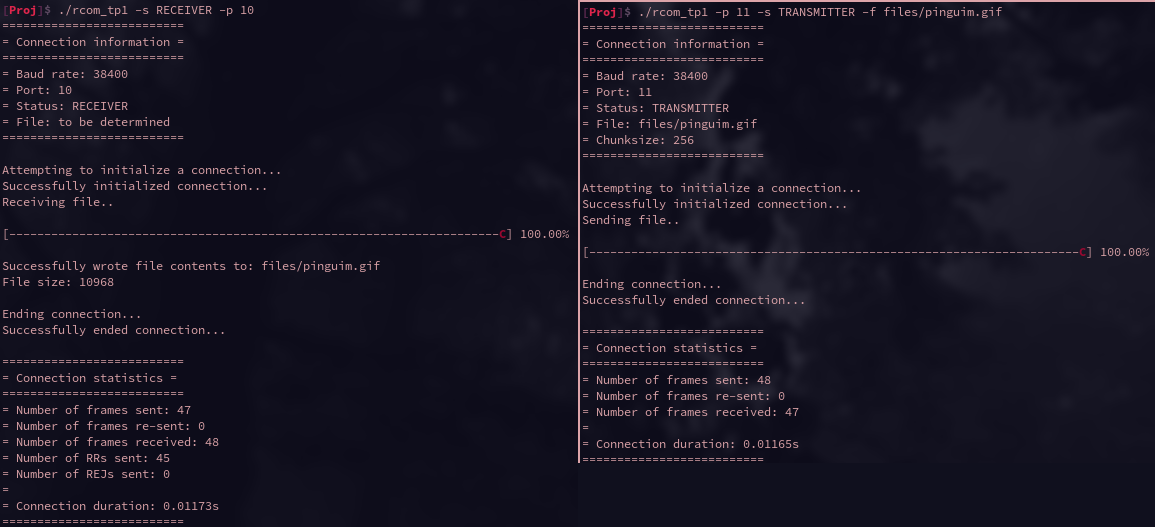
\includegraphics[width=0.8\columnwidth]{images/validacao1.png}}

Neste caso passámos o ficheiro pinguim.gif com um \textit{chunk size} diferente.
\centering{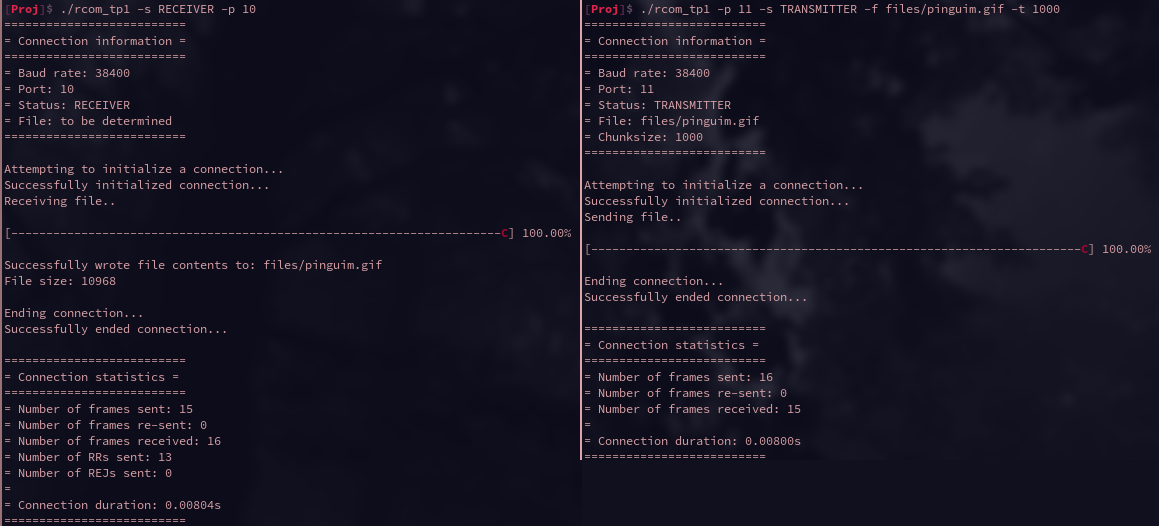
\includegraphics[width=0.8\columnwidth]{images/validacao2.png}}

Neste caso passámos o ficheiro pinguim.gif com um \textit{baud rate} diferente e
introdução artificial de erros.
\centering{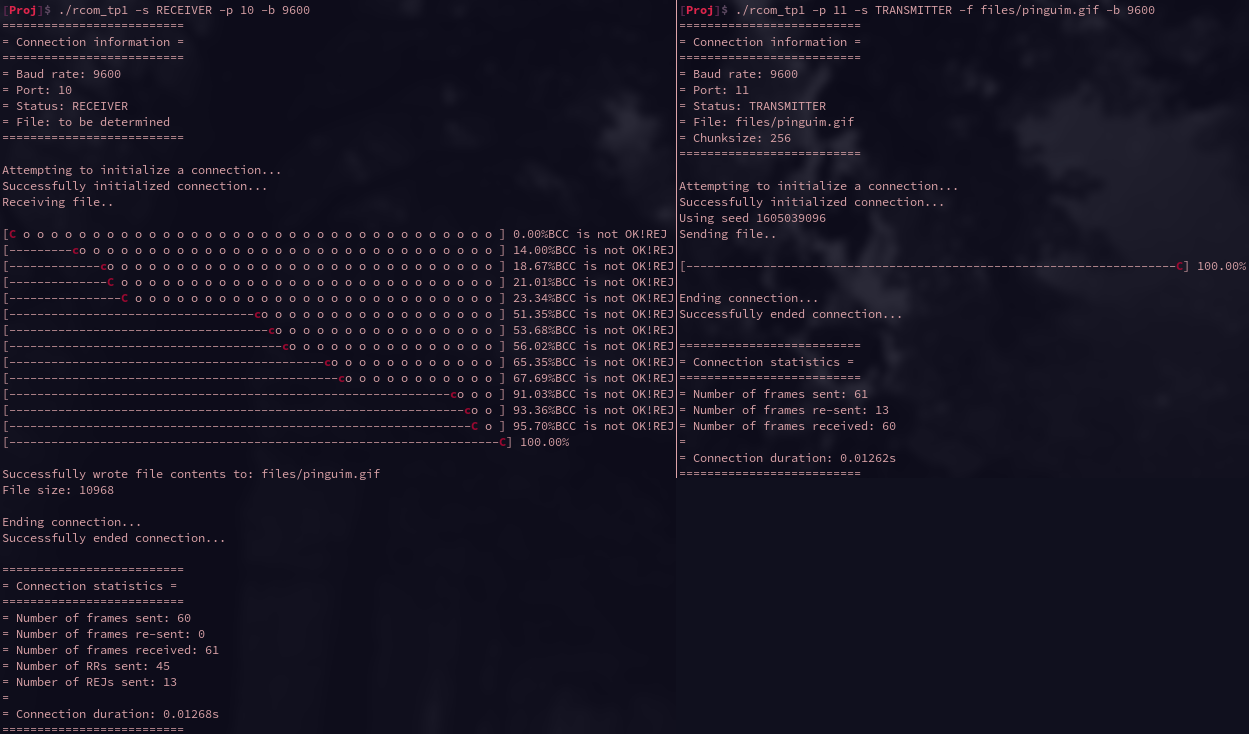
\includegraphics[width=0.8\columnwidth]{images/validacao3.png}}

\chapter{Eficiência do protocolo de ligação de dados}

\subsection{Tempo de propagação}

Com o objetivo de medir de forma fiável a eficiência do protocolo, foi calculado
o tempo de propagação $T_{prop}$ através da fórmula
$T_{prop} = T_{absRecebido} - T_{absEnviado}$. Sendo $T_{absRecebido}$ e $T_{absEnviado}$ o tempo
absoluto de envio do byte de teste, e o tempo de receção do byte de teste, respetivamente.

\begin{table}[h!]
  \begin{center}
    \caption{Cálculo do tempo de propagação médio}
    \label{tab:table1}
    \begin{tabular}{l|c|r|r} % <-- Alignments: 1st column left, 2nd middle and 3rd right, with vertical lines in between
        \textbf{$T_{absEnviado}(ns)$} &\textbf{$T_{absRecebido}(ns)$} & \textbf{$T_{prop}(ns)$} & \textbf{$\mu T_{prop}$}\\
      \hline
      267368335 & 264536179 & 2832156\\
      469990377 & 467159729 & 2830648\\
        672241506 & 669431417 & 2810089 & 2819355\\
      874435168 & 871625091 & 2810077\\
      77204397 & 74385042 & 2819355\\
    \end{tabular}
  \end{center}
\end{table}

\subsection{Análise de eficiência}

De modo a obter resultados mais precisos foram efetuados três medições
para cada cálculo do tempo de execução. As medições foram feitas remotamente
nos computadores laboratoriais da sala I320. Em cada medição foi usado um
\textit{chunksize} de 256 Bytes (a não ser que seja indicado o contrário)
e o ficheiro usado foi o fornecido no moodle da unidade curricular
(pinguim.gif).
\begin{table}[h!]
  \begin{center}
    \caption{Cálculo da eficiência sem introdução de erros}
    \label{tab:table1}
    \begin{tabular}{l|c|c} % <-- Alignments: 1st column left, 2nd middle and 3rd right, with vertical lines in between
        Baudrate & \textbf{$  T_{envio} (s) $} & S \\
      \hline
        9600 & 12.23109 & 0.98063\\
        19200 & 6.11795 & 0.96201\\
        38400 & 3.06131 & 0.92686\\
        57600 & 2.04245 & 0.89423\\
        115200 & 1.02359 & 0.80905\\
    \end{tabular}
  \end{center}
\end{table}

\begin{table}[h!]
  \begin{center}
    \caption{Cálculo da eficiência com introdução de erros}
    \label{tab:table1}
    \begin{tabular}{l|c|c|c|c} % <-- Alignments: 1st column left, 2nd middle and 3rd right, with vertical lines in between
        Baudrate & \textbf{$  T_{envio} (s) $} & Nº pacotes enviados & Nº pacotes reenviados & S\\
      \hline
        9600 & 15.11709 & 60.00000 & 12.00000 & 0.98427\\
        19200 & 7.11741 & 56.00000 & 8.00000 & 0.96717\\
        38400 & 4.08493 & 63.00000 & 15.00000 & 0.94416\\
        57600 & 2.55259 & 59.33333 & 11.33333 & 0.91354\\
        115200 & 1.43659 & 68.00000 & 20.00000 & 0.85604\\
    \end{tabular}
  \end{center}
\end{table}

\begin{table}[h!]
  \begin{center}
    \caption{Cálculo da eficiência com variação do chunksize}
    \label{tab:table1}
    \begin{tabular}{l|c|c} % <-- Alignments: 1st column left, 2nd middle and 3rd right, with vertical lines in between
        Chunksize & \textbf{$  T_{envio} (s) $} & S \\
      \hline
        1 & 58.20041 & 0.48482 \\
        10 & 8.42766 & 0.57676\\
        100 & 3.44801 & 0.84791\\
        1000 & 2.94857 & 0.97946\\
        10000 & 2.90310 & 0.99787\\
    \end{tabular}
  \end{center}
\end{table}

Nota: o tempo de propagação ($T_{prop}$) descrito na tabela abaixo é o valor
acrescido ao $T_{prop}$ da \textit{serial port}: \textbf{2820465.0 ns}.
\begin{table}[h!]
  \begin{center}
    \caption{Cálculo da eficiência com variação tempo de propagação}
    \label{tab:table1}
    \begin{tabular}{l|c|c} % <-- Alignments: 1st column left, 2nd middle and 3rd right, with vertical lines in between
        Tempo de propagação acrescido ($\mu s$) & \textbf{$  T_{envio} (s) $} & S \\
      \hline
        10 & 1.02574 & 0.80883\\
        100 & 1.85891 & 0.88139\\
        200 & 3.00061 & 0.92062\\
        500 & 6.45144 & 0.95777\\
        1000 & 12.271156 & 0.97402\\
    \end{tabular}
  \end{center}
\end{table}

\begin{table}[h!]
  \begin{center}
    \caption{Cálculo da eficiência com variação do tamanho do ficheiro}
    \label{tab:table1}
    \begin{tabular}{l|c|c} % <-- Alignments: 1st column left, 2nd middle and 3rd right, with vertical lines in between
        Tamanho do ficheiro ($bytes$) & \textbf{$  T_{envio} (s) $} & S\\
      \hline
        8 & 0.03026 & 0.99421\\
        10968 & 3.06077 & 0.92685\\
        239765 & 66.29077 & 0.92621\\
    \end{tabular}
  \end{center}
\end{table}

\chapter{Graphs}
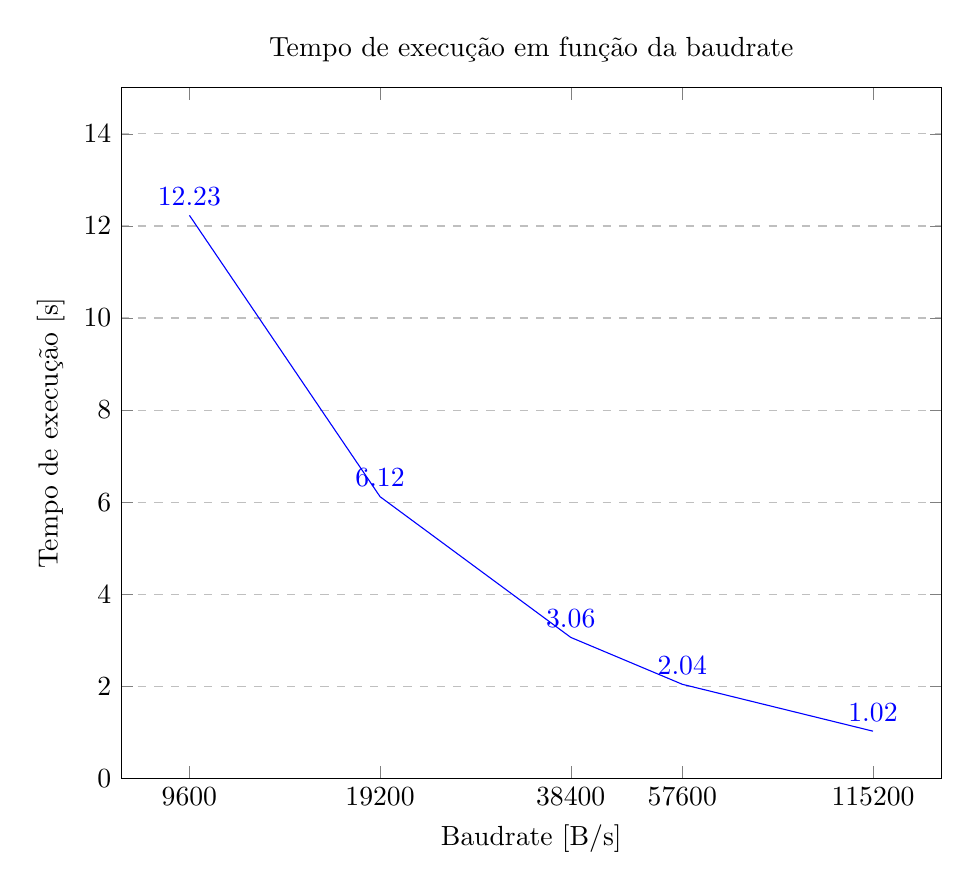
\begin{tikzpicture}
\begin{axis}[
    title={Tempo de execução em função da baudrate},
    width=12cm,
    xlabel={Baudrate [B/s]},
    ylabel={Tempo de execução [s]},
    ymin=0, ymax=15,
    xmode=log,
    xtick={9600, 19200, 38400, 57600, 115200},
    xticklabels={9600, 19200, 38400, 57600, 115200},
    legend pos=north west,
    ymajorgrids=true,
    grid style=dashed,
    nodes near coords,
]

\addplot[
    color=blue,
    ]
    coordinates {
        (9600, 12.23109)
        (19200, 6.11795)
        (38400, 3.06131)
        (57600, 2.04245)
        (115200, 1.02359)
    };
\end{axis}
\end{tikzpicture}

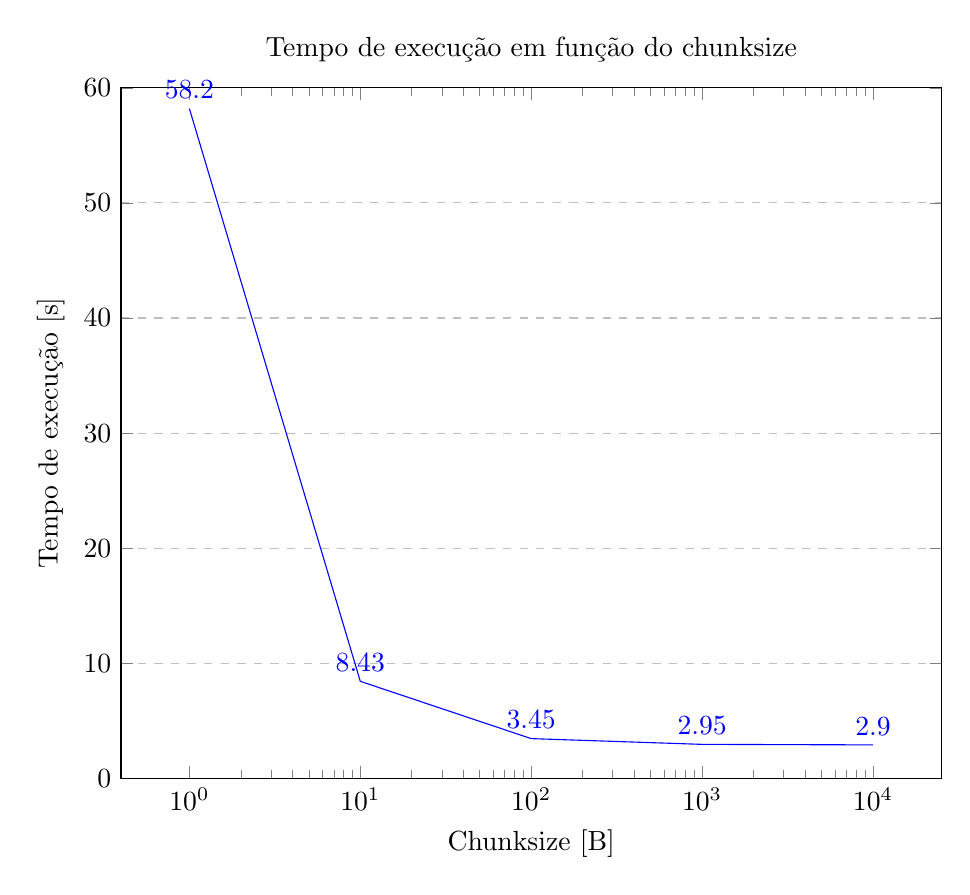
\begin{tikzpicture}
\begin{axis}[
    title={Tempo de execução em função do chunksize},
    width=12cm,
    xlabel={Chunksize [B]},
    ylabel={Tempo de execução [s]},
    ymin=0, ymax=60,
    xmode=log,
    xtick={1, 10, 100, 1000, 10000},
    legend pos=north west,
    ymajorgrids=true,
    grid style=dashed,
    nodes near coords,
]

\addplot[
    color=blue,
    ]
    coordinates {
        (1 , 58.20041)
        (10 , 8.42766)
        (100 , 3.44801)
        (1000 , 2.94857)
        (10000 , 2.90310)
    };
\end{axis}
\end{tikzpicture}

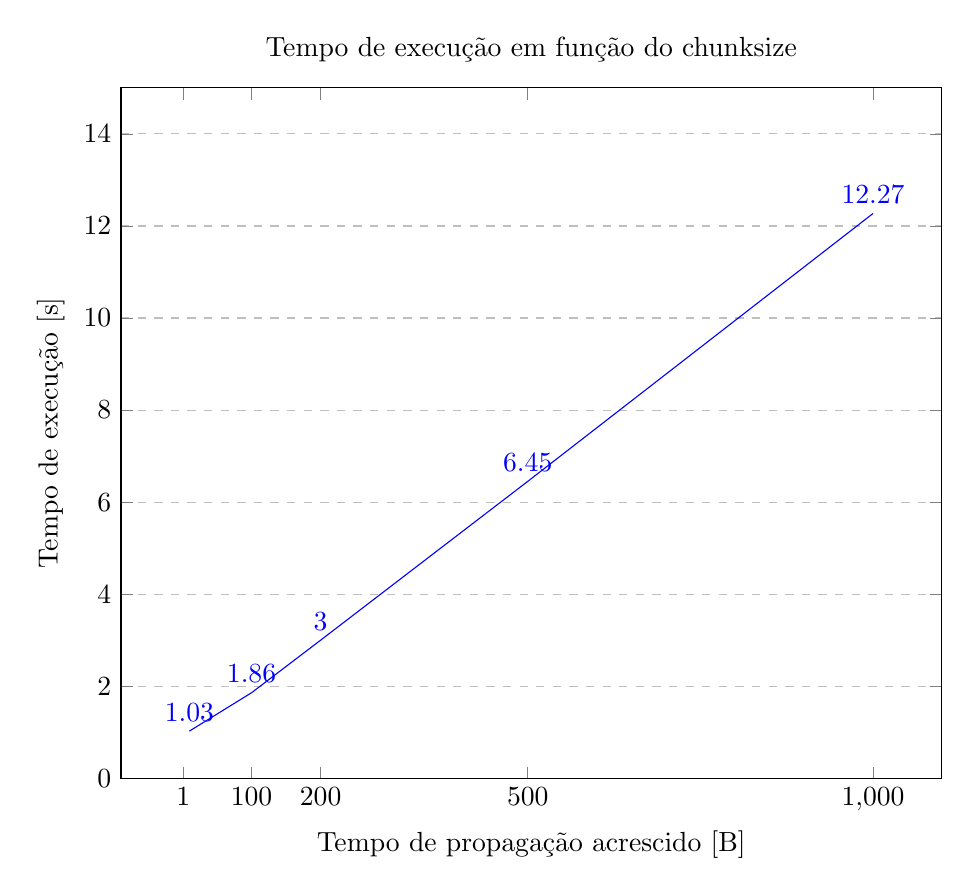
\begin{tikzpicture}
\begin{axis}[
    title={Tempo de execução em função do chunksize},
    width=12cm,
    xlabel={Tempo de propagação acrescido [B]},
    ylabel={Tempo de execução [s]},
    ymin=0, ymax=15,
    xtick={1, 100, 200, 500, 1000},
    legend pos=north west,
    ymajorgrids=true,
    grid style=dashed,
    nodes near coords,
]

\addplot[
    color=blue,
    ]
    coordinates {
        (10 , 1.02574)
        (100 , 1.85891)
        (200 , 3.00061)
        (500 , 6.45144)
        (1000 , 12.271156)
    };
\end{axis}
\end{tikzpicture}


O grupo planeava efetuar um maior número de medidas com um FER
maior, mas tal não foi possível pelo facto da conexão aos computadores
da FEUP ser muito fraca.
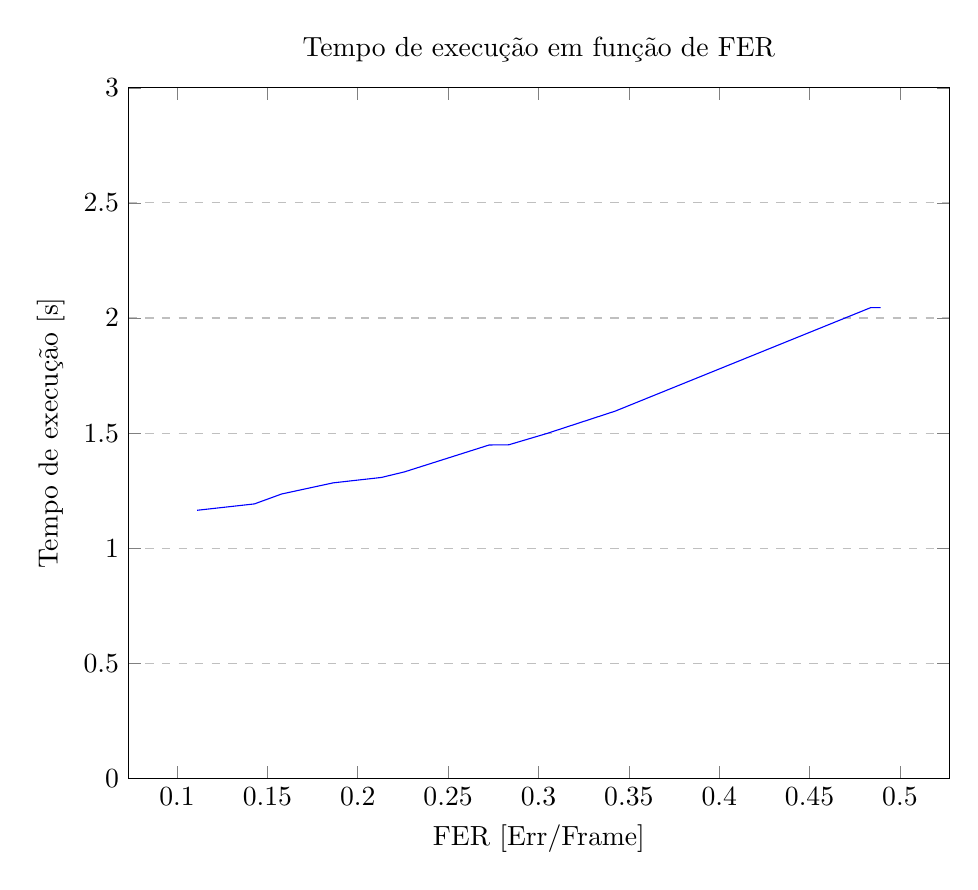
\begin{tikzpicture}
\begin{axis}[
    title={Tempo de execução em função de FER},
    width=12cm,
    xlabel={FER [Err/Frame]},
    ylabel={Tempo de execução [s]},
    ymin=0, ymax=3,
    legend pos=north west,
    ymajorgrids=true,
    grid style=dashed,
]

\addplot[
    color=blue,
    ]
    coordinates {
        (0.11111 , 1.16461)
        (0.14286 , 1.19231)
        (0.15789 , 1.23536)
        (0.18644 , 1.28378)
        (0.21311 , 1.30724)
        (0.22581 , 1.33135)
        (0.27273 , 1.44835)
        (0.28358 , 1.44912)
        (0.30435 , 1.49755)
        (0.34247 , 1.59548)
        (0.48387 , 2.04525)
        (0.48936 , 2.04511)
    };
\end{axis}
\end{tikzpicture}

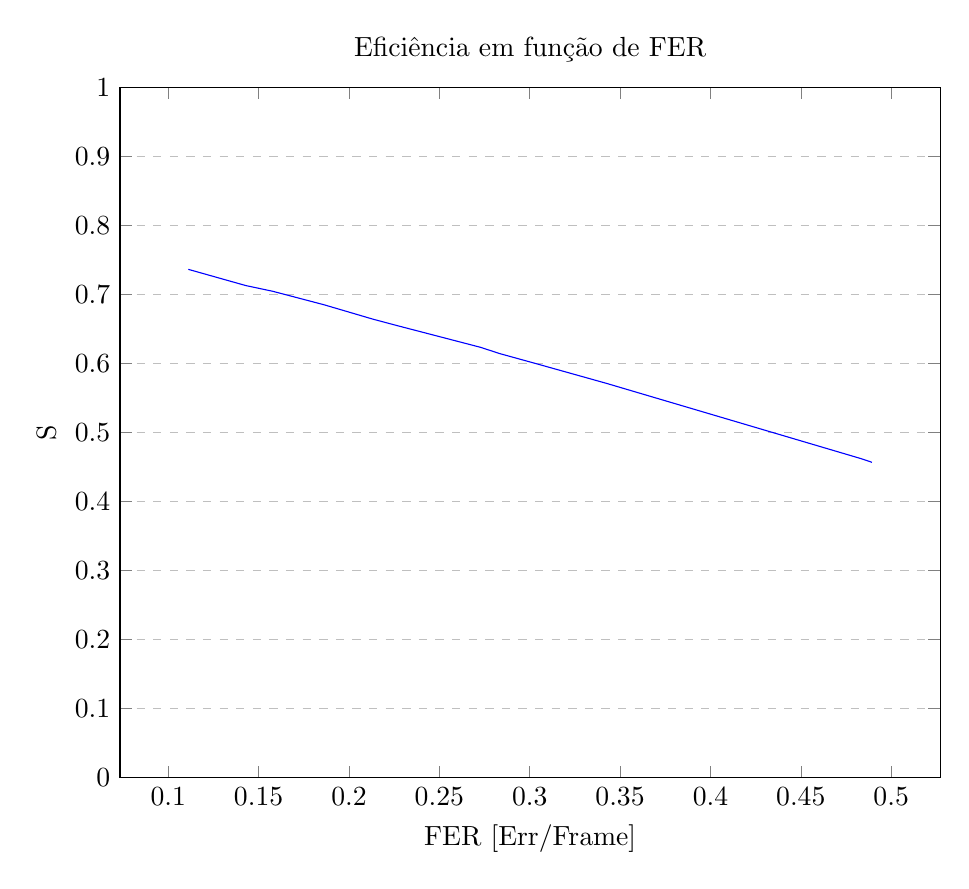
\begin{tikzpicture}
\begin{axis}[
    title={Eficiência em função de FER},
    width=12cm,
    xlabel={FER [Err/Frame]},
    ylabel={S},
    ymin=0, ymax=1,
    legend pos=north west,
    ymajorgrids=true,
    grid style=dashed,
]

\addplot[
    color=blue,
    ]
    coordinates {
        (0.11111 ,0.73618)
        (0.14286 ,0.71273)
        (0.15789 ,0.70437)
        (0.18644 ,0.68471)
        (0.21311 ,0.66415)
        (0.22581 ,0.65528)
        (0.27273 ,0.62330)
        (0.28358 ,0.61405)
        (0.30435 ,0.59902)
        (0.34247 ,0.57106)
        (0.48387 ,0.46161)
        (0.48936 ,0.45669)
    };
\end{axis}
\end{tikzpicture}

\chapter{Conclusões}

O aumento do valor do \textit{baud rate} resulta sempre em envios mais rápidos,
e vice-versa.

Em circunstâncias em que a probabilidade de ocorrência de erros é baixa
(\textbf{FER} baixo), o aumento do \textit{chunk size} (e consequente aumento
do tamanho das tramas) resulta em transferência mais rápidas. Este efeito é
mais evidente quando se realiza a comparação entre dois valores baixos de
\textit{chunk size}. É de notar que em casos em que o \textbf{FER} é alto,
o aumento do valor de \textit{chunk size} resultará em transferências mais
lentas, pois a quantidade de bytes a retransmitir a cada falha será maior.

\chapter*{Anexo A}
\addcontentsline{toc}{chapter}{Anexo A}

\section{Makefile}

\begin{lstlisting}
NAME = rcom_tp1
SRC = rcom_tp1.c app_layer.c app_layer_priv.c data_link.c data_link_priv.c vector.c
OBJ = ${SRC:.c=.o}

# compiler and linker
CC = gcc
# flags
CFLAGS = -lm -Wall -Wextra -DHASPROGRESS

all: options rcom

options:
	@echo rcom build options:
	@echo "CFLAGS = ${CFLAGS}"
	@echo "CC     = ${CC}"

.c.o:
	${CC} -c ${CFLAGS} $<

rcom: ${OBJ}
	${CC} ${CFLAGS} -o ${NAME} ${OBJ}

clean:
	rm -f ${NAME} ${OBJ}

test: clean all
	@make && ./rcom_tp1 -p 10 -s RECEIVER &
	sleep 0.1
	@./rcom_tp1 -p 11 -s TRANSMITTER -f files/gato.gif
	diff -q files/gato.gif out/files/gato.gif

.PHONY: all options clean rcom
\end{lstlisting}

\section{app\_layer.c}

\begin{lstlisting}
#include <fcntl.h>
#include <stdio.h>
#include <stdlib.h>
#include <string.h>
#include <sys/stat.h>
#include <unistd.h>

#include "app_layer_priv.h"
#include "data_link.h"

#define PROGRESSSIZE 70

static struct linkLayer linkLayer;
static struct termios oldtio;

void initAppLayer(struct applicationLayer *appLayer, int baudrate,
                  long chunksize) {
  linkLayer = initLinkLayer(); // TODO check errors

  appLayer->chunksize = chunksize;
  if (setBaudRate(&linkLayer, baudrate) < 0)
    fprintf(stderr, "Invalid baudrate. Using default: %d\n", DFLTBAUDRATE);
}

int llopen(int porta, enum applicationStatus appStatus) {
  /*
    Open serial port device for reading and writing and not as controlling tty
    because we don't want to get killed if linenoise sends CTRL-C.
  */
  char port_str[20];
  sprintf(port_str, "%d", porta);
  strcpy(linkLayer.port, PORTLOCATION);
  strcat(linkLayer.port, port_str);

  int fd = open(linkLayer.port, O_RDWR | O_NOCTTY);
  if (fd < 0) {
    perror(linkLayer.port);
    return -1;
  }

  if (tcgetattr(fd, &oldtio) == -1) { /* save current port settings */
    perror("tcgetattr");
    return -2;
  }

  struct termios newtio;
  bzero(&newtio, sizeof(newtio));
  newtio.c_cflag = linkLayer.baudRate | CS8 | CLOCAL | CREAD;
  newtio.c_iflag = IGNPAR;
  newtio.c_oflag = 0;

  /* set input mode (non-canonical, no echo,...) */
  newtio.c_lflag = 0;

  /*
    VTIME e VMIN devem ser alterados de forma a proteger com um temporizador a
    leitura do(s) proximo(s) caracter(es)
  */
  newtio.c_cc[VTIME] = MYVTIME; /* inter-unsigned character timer unused */
  newtio.c_cc[VMIN] = MYVMIN;   /* blocking read until X chars received */
  // clear queue
  tcflush(fd, TCIOFLUSH);

  // set new struct
  if (tcsetattr(fd, TCSANOW, &newtio) == -1) {
    perror("tcsetattr");
    return -3;
  }

  // handshake (receiver starts first)
  // SET ->
  // UA <-
  if (appStatus == RECEIVER) {
    if (initConnection(&linkLayer, fd, true) < 0)
      return -5;
  } else if (appStatus == TRANSMITTER) {
    if (initConnection(&linkLayer, fd, false) < 0)
      return -5;
  } else {
    return -4;
  }

  return fd;
}

int llwrite(int fd, char *buffer, int length) {
  if (sendFrame(&linkLayer, fd, (unsigned char *)buffer, length) < 0)
    return -1;
  return 0;
}

int llread(int fd, char **buffer) {
  int packet_length = getFrame(&linkLayer, fd, (unsigned char **)buffer);

  if (packet_length == 0)
    return 0; // Morreu so neste
  else if (packet_length < 0)
    return -1; // Morreu mesmo

  return packet_length;
}

int llclose(int fd, enum applicationStatus appStatus) {
  if (appStatus == RECEIVER) {
    if (endConnection(&linkLayer, fd, true))
      return -1;
  } else if (appStatus == TRANSMITTER) {
    if (endConnection(&linkLayer, fd, false))
      return -1;
  } else {
    return -2;
  }

  /* Reset serial port */
  sleep(1); // for safety (in case the transference is still on-going)
  if (tcsetattr(fd, TCSANOW, &oldtio) == -1) {
    perror("tcsetattr");
    return -3;
  }

  return close(fd);
}

long getStartPacketFileSize() {
  long file_size;
  memcpy(&file_size, getStartPacket() + 3, sizeof(long));
  return file_size;
}

int getStartPacketFileName(char **file_name) {
  *file_name = (char *)(getStartPacket() + 2 + sizeof(long) + 3);
  return (int)*(getStartPacket() + 2 + sizeof(long) + 2);
}

void drawProgress(float currPerc, int divs, bool isRedraw) {
#ifndef HASPROGRESS
  return;
#endif
  static int prev_full = -1;
  int full = (int)(currPerc * divs);
  if (full < 0)
    full = 0;
  else if (full > divs)
    full = divs;

  if (full == prev_full)
    return;
  prev_full = full;

  /* draw */
  if (isRedraw) {
    for (int i = 0; i < divs + 10; ++i)
      printf("\b");
  }

  printf("[");
  for (int i = 0; i < full; ++i)
    printf("-");
  printf("\33\[33m\33\[1m");
  printf(full % 2 == 0 ? "C" : "c");
  printf("\33\[0m");
  for (int i = full + 1; i < divs; ++i)
    printf(i % 2 == 0 ? "o" : " ");
  printf("] %.2f%%", currPerc * 100);

  fflush(stdout);
}

int sendFile(struct applicationLayer *appLayer) {
  printf("Sending file..\n");

  FILE *fp = fopen(appLayer->file_name, "rb");
  if (fp == NULL) {
    perror(appLayer->file_name);
    return -1;
  }

  struct stat sb;
  if (stat(appLayer->file_name, &sb) == -1) {
    perror("stat");
    return -1;
  }
  appLayer->file_size = sb.st_size;

  unsigned char *file_content =
      (unsigned char *)malloc(sizeof(unsigned char) * appLayer->file_size);
  if (appLayer->file_size > 0) { // empty file
    if (fread(file_content, sizeof(unsigned char), appLayer->file_size, fp) ==
        0) {
      perror("sendfile() read");
      return -2;
    }
  }

  // Send start control packet
  unsigned char *start_packet = NULL;
  int start_length = assembleControlPacket(appLayer, false, &start_packet);
  if (llwrite(appLayer->fd, (char *)start_packet, start_length) < 0) {
    free(start_packet);
    return -3;
  }

  puts("");
  drawProgress(0, PROGRESSSIZE, false);
  // Send info packets
  long ind = 0, trSize = 0;
  while (ind < appLayer->file_size) {
    // send info fragment
    unsigned char *packet = NULL;
    int length;
    if (appLayer->file_size - ind >= appLayer->chunksize) {
      length = assembleInfoPacket((char *)file_content + ind,
                                  appLayer->chunksize, &packet);
      trSize += appLayer->chunksize;
    } else {
      length = assembleInfoPacket((char *)file_content + ind,
                                  appLayer->file_size - ind, &packet);
      trSize += appLayer->file_size - ind;
    }

    if (llwrite(appLayer->fd, (char *)packet, length) < 0) {
      free(packet);
      return -4;
    }

    drawProgress((float)trSize / appLayer->file_size, PROGRESSSIZE, true);
    free(packet);
    ind += appLayer->chunksize;
  }

  // Send end control packet
  unsigned char *end_packet = NULL;
  int end_length = assembleControlPacket(appLayer, true, &end_packet);
  if (llwrite(appLayer->fd, (char *)end_packet, end_length) < 0) {
    free(end_packet);
    return -5;
  }

  drawProgress(100, PROGRESSSIZE, true);
  puts("");

  return appLayer->file_size;
}

int receiveFile(struct applicationLayer *appLayer, unsigned char **res) {
  printf("Receiving file..\n");

  unsigned char *buf = NULL;
  bool stop = false;
  do {
    int n = llread(appLayer->fd, (char **)&buf);
    if (n < 0) {
      fprintf(stderr, "Morreu mesmo.\n");
      return -1;
    } else if (n == 0) { // Invalid packet, try again
      stop = false;
    } else {
      int status = parsePacket(buf, n);
      if (status < 0)
        fprintf(stderr, "Invalid packet formatting.\n");
      else if (status == C_START)
        stop = true;
      else
        stop = false;
    }

  } while (!stop);

  long fileSize = getStartPacketFileSize();
  *res = (unsigned char *)malloc(sizeof(unsigned char) * fileSize);

  puts("");
  drawProgress(0, PROGRESSSIZE, false);
  stop = false;
  int curr_file_n = 0;
  while (!stop) {
    int n = llread(appLayer->fd, (char **)&buf);

    if (n < 0) {
      perror("Morreu mesmo");
      return -1;
    } else if (n == 0) {
      stop = false;
    } else {
      int status = parsePacket(buf, n);
      if (status < 0)
        fprintf(stderr, "Invalid packet formatting.\n");
      else if (status == C_END)
        stop = true;
      else if (status == C_DATA) {
        memcpy(*res + curr_file_n, buf + 4, n - 4);
        free(buf);
        curr_file_n += n - 4;
        stop = false;
      } else
        stop = false;
      drawProgress((float)curr_file_n / fileSize, PROGRESSSIZE, true);
    }
  }

  drawProgress(1, PROGRESSSIZE, true);
  puts("");
  return 0;
}

void write_file(struct applicationLayer *appLayer,
                unsigned char *file_content) {
  /*
   * struct stat st;
   * if (stat("out/", &st) == -1) {
   *   mkdir("out", 0770);
   * }
   */

  char out_file[512];
  if (strcmp(appLayer->file_name, "")) { // not empty
    stpcpy(out_file, appLayer->file_name);
  } else {
    strcpy(out_file, "");
    char *file_name;
    int file_name_size = getStartPacketFileName(&file_name);
    strncat(out_file, file_name, file_name_size);
  }

  FILE *fp = fopen(out_file, "w+b");
  if (fp == NULL) {
    perror("Failed creating output file");
  } else {
    if (fwrite(file_content, sizeof(unsigned char), getStartPacketFileSize(),
               fp) == 0) {
      perror("Failed writting");
    } else {
      printf("\nSuccessfully wrote file contents to: %s\nFile size: %ld\n",
             out_file, getStartPacketFileSize());
    }
    fclose(fp);
  }
}

void printConnectionStats(enum applicationStatus status) {
  struct linkStats *stats = &linkLayer.stats;

  puts("\n==========================\n= Connection statistics "
       "=\n==========================");
  printf("= Number of frames sent: %d\n", stats->sent);
  printf("= Number of frames re-sent: %d\n", stats->resent);
  printf("= Number of frames received: %d\n", stats->received);
  if (status == RECEIVER) {
    printf("= Number of RRs sent: %d\n", stats->RRs);
    printf("= Number of REJs sent: %d\n", stats->REJs);
  }

  double result =
      stats->end_time.tv_sec - stats->start_time.tv_sec +
      ((stats->end_time.tv_nsec - stats->start_time.tv_nsec) / 1000000000.0);
  printf("=\n= Connection duration: %.5lfs\n", result);
  puts("==========================");
}
\end{lstlisting}

\section{app\_layer.h}

\begin{lstlisting}
#ifndef APPLAYER_H
#define APPLAYER_H

#include <stdbool.h>
#include <termios.h>

#define PORTLOCATION "/dev/ttyS"

enum applicationStatus { TRANSMITTER, RECEIVER, NONE };

struct applicationLayer {
  int fd; /* file descriptor correspondente a porta serie */
  enum applicationStatus status; /* TRANSMITTER or RECEIVER */
  char file_name[256];           /* name of file to transmit (if any) */
  long file_size;                /* size of file to transmit (if any) */
  long chunksize;                /* tansmission chunksize */
};

void initAppLayer(struct applicationLayer *appLayer, int baudrate,
                  long chunksize);

int llopen(int porta, enum applicationStatus appStatus);

int llwrite(int fd, char *buffer, int length);

int llread(int fd, char **buffer);

int llclose(int fd, enum applicationStatus appStatus);

long getStartPacketFileSize();
int getStartPacketFileName(char **file_name);

int sendFile(struct applicationLayer *appLayer);
int receiveFile(struct applicationLayer *appLayer, unsigned char **res);
void write_file(struct applicationLayer *appLayer, unsigned char *file_content);

void printConnectionStats(enum applicationStatus status);

#endif // APPLAYER_H
\end{lstlisting}

\section{app\_layer\_priv.c}

\begin{lstlisting}
#include <stdio.h>
#include <stdlib.h>
#include <string.h>

#include "app_layer_priv.h"

static unsigned char *startPacket;

int assembleControlPacket(struct applicationLayer *appLayer, bool is_end,
                          unsigned char **buf) {
  // C = 2/3 | T1 - L1 - V1 | T2 - L2 - V2 | ...
  // T (type): 0 tamanho file, 1 nome file, etc...
  // L (byte): length
  // V: valor (L length bytes)

  /* assemble packet */
  unsigned char *packet;
  int file_name_len = strlen(appLayer->file_name);
  int length = 1 + 2 + file_name_len + 2 + sizeof(long);
  packet = (unsigned char *)malloc(length * sizeof(unsigned char));
  if (packet == NULL) {
    perror("App layer packet instantiation");
    return -1;
  }

  int curr_ind = 0;
  if (is_end)
    packet[curr_ind++] = C_END;
  else
    packet[curr_ind++] = C_START;

  // TLV file size
  packet[curr_ind++] = T_SIZE;
  packet[curr_ind++] = sizeof(long);
  memcpy(packet + curr_ind, &appLayer->file_size, sizeof(long));
  curr_ind += sizeof(long);

  // TLV file name
  packet[curr_ind++] = T_NAME;
  packet[curr_ind++] = file_name_len;
  memcpy(packet + curr_ind, appLayer->file_name, file_name_len);
  *buf = packet;

  return length;
}

int assembleInfoPacket(char *buffer, int length, unsigned char **res) {
  // C = 1 | N | L2 - L1: 256 * L2 + L1 = k | P1..Pk (k bytes)
  /* assemble packet */
  static unsigned char n =
      MAXSEQNUM; // unsigned integer overflow is defined >:(
  ++n;

  int new_length = length + 4;
  unsigned char *packet =
      (unsigned char *)malloc(new_length * sizeof(unsigned char));
  if (packet == NULL) {
    perror("App layer packet instantiation");
    return -1;
  }

  packet[C_CONTROL] = C_DATA;
  packet[SEQ_NUMBER] = n;
  packet[L2] = (unsigned char)(length / L2VAL);
  packet[L1] = (unsigned char)(length % L2VAL);
  memcpy(packet + 4, buffer, sizeof(char) * length);

  *res = packet;
  return new_length;
}

int parseControlPacket(unsigned char *packet) {
  int curr_ind = C_CONTROL + 1;
  int size_type = packet[curr_ind++];
  if (size_type != T_SIZE) {
    fprintf(stderr, "Invalid size type %d\n", size_type);
    return -1;
  }

  int size_length = packet[curr_ind++];
  curr_ind += size_length;

  int name_type = packet[curr_ind++];
  if (name_type != T_NAME) {
    fprintf(stderr, "Invalid name type %d\n", name_type);
    return -1;
  }

  if (packet[C_CONTROL] == C_START)
    startPacket = packet;

  return 0;
}

int parsePacket(unsigned char *packet, int packet_length) {
  // unsigned integer overflow is defined >:(
  static unsigned char n = 0;

  if (packet[C_CONTROL] == C_DATA) { // Verifications in case of data
    if (packet[SEQ_NUMBER] != n) { // Invalid sequence number
      fprintf(stderr, "Sq num: %d->%d\n", packet[SEQ_NUMBER], n);
      free(packet);
      return -2;
    }
    ++n;

    int expected_length = packet[L2] * L2VAL + packet[L1] + 4;
    if (expected_length != packet_length) {
      fprintf(stderr, "Invalid length: %d->%d\n", expected_length,
              packet_length);
      free(packet);
      return -2;
    }

  } else if (packet[C_CONTROL] == C_START ||
             packet[C_CONTROL] == C_END) { // Start and End

    if (parseControlPacket(packet) < 0) {
      free(packet);
      return -3;
    }

  } else {
    fprintf(stderr, "Seq header %d\n", packet[C_CONTROL]);
    free(packet);
    return -3; // Unexpected C header
  }

  return packet[C_CONTROL];
}

unsigned char *getStartPacket() { return startPacket; }
\end{lstlisting}

\section{app\_layer\_priv.h}

\begin{lstlisting}
#ifndef APPLAYER_PRIV_H
#define APPLAYER_PRIV_H

#define C_DATA 1
#define C_START 2
#define C_END 3
#define L2VAL 256
#define T_SIZE 0
#define T_NAME 1

/* Packet Headers */
#define C_CONTROL 0
#define SEQ_NUMBER 1
#define L2 2
#define L1 3
#define MAXSEQNUM 255

#define MYVTIME 1
#define MYVMIN 0

#include "app_layer.h"

int assembleControlPacket(struct applicationLayer *appLayer, bool is_end,
                          unsigned char **buffer);
int assembleInfoPacket(char *buffer, int length, unsigned char **packet);

int parseControlPacket(unsigned char *packet);
int parsePacket(unsigned char *packet, int packet_length);
bool isEndPacket(unsigned char *packet, int n);
unsigned char *getStartPacket();

#endif // APPLAYER_PRIV_H
\end{lstlisting}

\section{data\_link.c}

\begin{lstlisting}
#include <stdio.h>

#include "data_link_priv.h"

int initConnection(struct linkLayer *linkLayer, int fd, bool isReceiver) {
  printf("\nAttempting to initialize a connection...\n");
  fflush(stdout);

  int failed = 0;
  if (isReceiver) {
    if (inputLoopSET(linkLayer, fd) < 0 || sendUAMsg(linkLayer, fd, true) < 0)
      failed = -1;
  } else {
    if (sendSetMsg(linkLayer, fd) < 0 || inputLoopUA(linkLayer, fd, false) < 0)
      failed = -1;
  }

  // save start time
  clock_gettime(CLOCK_REALTIME, &linkLayer->stats.start_time);

  if (!failed) {
    printf("Successfully initialized connection...\n");
    fflush(stdout);
  }

  return failed;
}

int endConnection(struct linkLayer *linkLayer, int fd, bool isReceiver) {
  printf("\nEnding connection...\n");
  fflush(stdout);

  int failed = 0;
  if (isReceiver) {
    if (inputLoopDISC(linkLayer, fd, true) < 0 ||
        sendDISCMsg(linkLayer, fd, true) < 0)
      failed = 1;
    if (inputLoopUA(linkLayer, fd, true) < 0)
      fprintf(stderr,
              "Didn't receive UA.. Assuming the disconnect was successful!\n");
  } else {
    if (sendDISCMsg(linkLayer, fd, false) < 0 ||
        inputLoopDISC(linkLayer, fd, false) < 0 ||
        sendUAMsg(linkLayer, fd, false) < 0)
      failed = 1;
  }

  clock_gettime(CLOCK_REALTIME, &linkLayer->stats.end_time);

  if (!failed) {
    printf("Successfully ended connection...\n");
    fflush(stdout);
  }

  return failed;
}

int setBaudRate(struct linkLayer *linkLayer, int baudrate) {
  switch (baudrate) {
  case 0:
    linkLayer->baudRate = B0;
    return B0;
  case 50:
    linkLayer->baudRate = B50;
    return B50;
  case 75:
    linkLayer->baudRate = B75;
    return B75;
  case 110:
    linkLayer->baudRate = B110;
    return B110;
  case 134:
    linkLayer->baudRate = B134;
    return B134;
  case 150:
    linkLayer->baudRate = B150;
    return B150;
  case 200:
    linkLayer->baudRate = B200;
    return B200;
  case 300:
    linkLayer->baudRate = B300;
    return B300;
  case 600:
    linkLayer->baudRate = B600;
    return B600;
  case 1200:
    linkLayer->baudRate = B1200;
    return B1200;
  case 1800:
    linkLayer->baudRate = B1800;
    return B1800;
  case 2400:
    linkLayer->baudRate = B2400;
    return B2400;
  case 4800:
    linkLayer->baudRate = B4800;
    return B4800;
  case 9600:
    linkLayer->baudRate = B9600;
    return B9600;
  case 19200:
    linkLayer->baudRate = B19200;
    return B19200;
  case 38400:
    linkLayer->baudRate = B38400;
    return B38400;
  case 57600:
    linkLayer->baudRate = B57600;
    return B57600;
  case 115200:
    linkLayer->baudRate = B115200;
    return B115200;
  case 230400:
    linkLayer->baudRate = B230400;
    return B230400;
  case 460800:
    linkLayer->baudRate = B460800;
    return B460800;
  default:
    linkLayer->baudRate = DFLTBAUDRATE;
    return -1;
  }
}
\end{lstlisting}

\section{data\_link.h}

\begin{lstlisting}
#ifndef DATALINK_H // TOOL - Schism
#define DATALINK_H

#include <stdbool.h>
#include <time.h>

#include "vector.h"

#define TIMEOUT 3 // seconds between answers
#define MAXATTEMPTS 3
#define DFLTBAUDRATE 38400

#define MAX_SIZE 256 // in Bytes

struct linkStats {
  unsigned int sent;          /* total number of sent frames */
  unsigned int resent;        /* number of resent frames */
  unsigned int received;      /* total number of received frames */
  unsigned int RRs;           /* number of RRs sent */
  unsigned int REJs;          /* number of REJs sent */
  struct timespec start_time; /* time at which the connection started */
  struct timespec end_time;   /* time at which the connection ended */
};

struct linkLayer {
  char port[20];                 /* Dispositivo /dev/ttySx, x = 0, 1 */
  int baudRate;                  /* Velcidade de transmissao */
  unsigned int sequenceNumber;   /* Numero de sequencia da trama: 0, 1*/
  unsigned int timeout;          /* Valor do temporizador, e.g.: 1 sec */
  unsigned int numTransmissions; /* Numero de retransmissoes em caso de falha */
  vector *frame;                 /* last sent frame */
  struct linkStats stats;        /* connection statistics */
};

struct linkLayer initLinkLayer();

int initConnection(struct linkLayer *linkLayer, int fd, bool isReceiver);
int endConnection(struct linkLayer *linkLayer, int fd, bool isReceiver);
int setBaudRate(struct linkLayer *linkLayer, int baudrate);

/* ret: < 0, error
 *      0, request resend of packet
 *      > 0, size of packet
 */
int getFrame(struct linkLayer *linkLayer, int fd, unsigned char **packet);

/* llwrite BACKEND */
int sendFrame(struct linkLayer *linkLayer, int fd, unsigned char *packet,
              int len);

#endif // DATALINK_H
\end{lstlisting}

\section{data\_link\_priv.c}

\begin{lstlisting}
#include <errno.h>
#include <signal.h>
#include <stdio.h>
#include <stdlib.h>
#include <string.h>
#include <unistd.h>

#include "data_link_priv.h"

static volatile bool needResend = false;

/* ALARM */
void alrmHandler(int signo) {
  if (signo != SIGALRM)
    return;

  needResend = true;
}

int resendHandler(struct linkLayer *linkLayer, int fd) {
  printf("RESEND\n");
  fflush(stdout);
  if (errno != EINTR || !needResend) // the failure wasn't caused by the alarm
    return -1;
  needResend = false;

  --linkLayer->numTransmissions;
  if (linkLayer->numTransmissions <= 0) {
    fprintf(stderr, "resendHandler(): Failed waiting for answer timedout\n");
    return -2;
  }

  ++linkLayer->stats.resent;
  if (sendAndAlarm(linkLayer, fd) < 0) {
    perror("Failed re-sending last message");
    return -3;
  }

  return 0;
}

/* WRITE FUNCTIONS */
int sendAndAlarm(struct linkLayer *linkLayer, int fd) {
  ++linkLayer->stats.sent;
  int res = write(fd, linkLayer->frame->data, linkLayer->frame->end);
  // set alarm
  alarm(linkLayer->timeout);
  return res;
}

int sendAndAlarmReset(struct linkLayer *linkLayer, int fd) {
  // reset attempts
  linkLayer->numTransmissions = MAXATTEMPTS;
  return sendAndAlarm(linkLayer, fd);
}

/* BASICS */
struct linkLayer initLinkLayer() {
  struct linkLayer linkLayer;
  setBaudRate(&linkLayer, DFLTBAUDRATE);
  linkLayer.sequenceNumber = 0;
  linkLayer.timeout = TIMEOUT;
  linkLayer.numTransmissions = MAXATTEMPTS;
  linkLayer.frame = new_vector();
  vec_reserve(linkLayer.frame, MAX_SIZE);

  struct linkStats *stats = &linkLayer.stats;
  stats->sent = 0;
  stats->resent = 0;
  stats->received = 0;
  stats->RRs = 0;
  stats->REJs = 0;

  /* Set alarm signal handler */
  struct sigaction sa;
  sa.sa_handler = alrmHandler;
  sigemptyset(&sa.sa_mask);
  sa.sa_flags = 0;
  if (sigaction(SIGALRM, &sa, NULL) == -1) {
    perror("setting alarm handler failed");
  }

  return linkLayer;
}

void fillByteField(unsigned char *buf, enum SUByteField field,
                   unsigned char byte) {
  buf[field] = byte;
}

unsigned char calcBCCField(unsigned char *buf) {
  return (buf[A_FIELD] ^ buf[C_FIELD]);
}

bool checkBCCField(unsigned char *buf) {
  return calcBCCField(buf) == buf[BCC_FIELD];
}

void setBCCField(unsigned char *buf) {
  unsigned char bcc = buf[A_FIELD] ^ buf[C_FIELD];
  fillByteField(buf, BCC_FIELD, bcc);
}

unsigned char calcBCC2Field(unsigned char *buf, int size) {
  unsigned char ret = 0;
  for (int i = 0; i < size; ++i)
    ret ^= buf[i];
  return ret;
}

bool checkBCC2Field(unsigned char *buf, int size) {
  return calcBCC2Field(buf, size) == buf[size];
}

/* STRING STUFFING */
int stuffByte(unsigned char byte, unsigned char res[]) {
  int bytes_returned = 1;
  if (byte == ESC) {
    res[0] = ESC;
    res[1] = ESC ^ STUFF_BYTE;
    bytes_returned = 2;
  } else if (byte == FLAG) {
    res[0] = ESC;
    res[1] = FLAG ^ STUFF_BYTE;
    bytes_returned = 2;
  } else
    res[0] = byte;
  return bytes_returned;
}

int stuffString(unsigned char *str, unsigned char *res, int size) {
  int j = 0;
  for (int i = 0; i < size; ++i) {
    unsigned char stuffedBytes[2];
    int n = stuffByte(str[i], stuffedBytes);
    res[j++] = stuffedBytes[0];
    if (n > 1)
      res[j++] = stuffedBytes[1];
  }
  return j;
}

unsigned char destuffByte(unsigned char byte) { return byte ^ STUFF_BYTE; }

/* PACKET ASSEMBLY */
void assembleSUFrame(struct linkLayer *linkLayer,
                     enum SUMessageType messageType) {
  fillByteField(linkLayer->frame->data, FLAG1_FIELD, FLAG);
  fillByteField(linkLayer->frame->data, A_FIELD, A_SENDER);
  fillByteField(linkLayer->frame->data, FLAG2_FIELD, FLAG);

  // set C_FIELD
  switch (messageType) {
  case SET_MSG:
    fillByteField(linkLayer->frame->data, C_FIELD, C_SET);
    break;
  case DISCSEND_MSG:
    fillByteField(linkLayer->frame->data, C_FIELD, C_DISC);
    break;
  case DISCRECV_MSG:
    fillByteField(linkLayer->frame->data, C_FIELD, C_DISC);
    fillByteField(linkLayer->frame->data, A_FIELD, A_RCV);
    break;
  case UASEND_MSG:
    fillByteField(linkLayer->frame->data, C_FIELD, C_UA);
    break;
  case UARECV_MSG:
    fillByteField(linkLayer->frame->data, C_FIELD, C_UA);
    fillByteField(linkLayer->frame->data, A_FIELD, A_RCV);
    break;
  case RR_MSG:
    fillByteField(linkLayer->frame->data, C_FIELD,
                  C_RR | (linkLayer->sequenceNumber << 7));
    break;
  case REJ_MSG:
    fillByteField(linkLayer->frame->data, C_FIELD,
                  C_REJ | (linkLayer->sequenceNumber << 7));
    break;
  default: // ?
    fillByteField(linkLayer->frame->data, C_FIELD, 0);
    break;
  }

  setBCCField(linkLayer->frame->data);
  linkLayer->frame->end = 5;
}

int assembleInfoFrame(struct linkLayer *linkLayer, unsigned char *buf,
                      int size) {
  fillByteField(linkLayer->frame->data, FLAG1_FIELD, FLAG);
  fillByteField(linkLayer->frame->data, A_FIELD, A_SENDER);
  fillByteField(linkLayer->frame->data, C_FIELD,
                (linkLayer->sequenceNumber << 6));
  setBCCField(linkLayer->frame->data);

  // in the worst case, every byte is stuffed
  unsigned char *stuffed_string =
      (unsigned char *)malloc(sizeof(unsigned char) * size * 2);
  if (stuffed_string == NULL) {
    perror("assembleInfoFrame malloc");
    return -1;
  }
  int new_size = stuffString(buf, stuffed_string, size);
  int i = HEADER_LEN;

  vec_reserve(linkLayer->frame,
              HEADER_LEN + new_size + 3); // BCC2 (x2) + end flag
  memcpy(linkLayer->frame->data + i, stuffed_string, new_size);
  free(stuffed_string);

  unsigned char bcc2_res[2], bcc2 = calcBCC2Field(buf, size);
  int bcc2_size = stuffByte(bcc2, bcc2_res);
  linkLayer->frame->data[new_size + (i++)] = bcc2_res[0];

  if (bcc2_size == 2)
    linkLayer->frame->data[new_size + (i++)] = bcc2_res[1];

  linkLayer->frame->data[new_size + i] = FLAG;

  linkLayer->frame->end = new_size + i + 1;
  return new_size + i;
}

/* STATE MACHINE */
transitions byteToTransitionSET(unsigned char byte, unsigned char *buf,
                                state curr_state) {
  transitions transition;
  if (curr_state == CS_ST && byte == calcBCCField(buf)) {
    transition = BCC_RCV;
  } else {
    switch (byte) {
    case FLAG:
      transition = FLAG_RCV;
      break;
    case A_SENDER: // == C_SET
      if (curr_state == FLAG_ST) {
        transition = A_RCV;
      } else if (curr_state == A_ST) {
        transition = CS_RCV;
      }
      break;
    default:
      transition = OTHER_RCV;
      break;
    }
  }

  return transition;
}

transitions byteToTransitionUA(unsigned char byte, unsigned char *buf,
                               state curr_state, bool isRecv) {
  transitions transition;
  if (curr_state == CS_ST && byte == calcBCCField(buf)) {
    transition = BCC_RCV;
  } else {
    switch (byte) {
    case FLAG:
      transition = FLAG_RCV;
      break;
    case A_RECEIVER:
      if (isRecv)
        transition = A_RCV;
      else
        transition = OTHER_RCV;
      break;
    case A_SENDER:
      if (!isRecv)
        transition = A_RCV;
      else
        transition = OTHER_RCV;
      break;
    case C_UA:
      transition = CS_RCV;
      break;
    default:
      transition = OTHER_RCV;
      break;
    }
  }

  return transition;
}

transitions byteToTransitionI(unsigned char byte, state curr_state) {
  transitions transition;
  if (curr_state == CI_ST) { // && byte == calcBCCField(buf)) {
    // TODO mandar REJ?
    transition = BCC_RCV;
  } else {
    switch (byte) {
    case FLAG:
      transition = FLAG_RCV;
      break;
    case A_SENDER:
      transition = A_RCV;
      break;
    case C_CTRL0:
    case C_CTRL1:
      transition = CI_RCV;
      break;
    default:
      transition = OTHER_RCV;
      break;
    }
  }

  return transition;
}

transitions byteToTransitionRR(unsigned char byte, unsigned char *buf,
                               state curr_state) {
  transitions transition;
  if (curr_state == CS_ST && byte == calcBCCField(buf)) {
    transition = BCC_RCV;
  } else {
    switch (byte) {
    case FLAG:
      transition = FLAG_RCV;
      break;
    case A_SENDER:
      transition = A_RCV;
      break;
    case C_RR:
    case C_RR | (1 << 7):
    case C_REJ:
    case C_REJ | (1 << 7):
      transition = CS_RCV;
      break;
    default:
      transition = OTHER_RCV;
      break;
    }
  }

  return transition;
}

transitions byteToTransitionDISC(unsigned char byte, unsigned char *buf,
                                 state curr_state, bool isRecv) {
  transitions transition;
  if (curr_state == CS_ST && byte == calcBCCField(buf)) {
    transition = BCC_RCV;
  } else {
    switch (byte) {
    case FLAG:
      transition = FLAG_RCV;
      break;
    case A_RECEIVER:
      if (!isRecv) // if we are receiver, we want the sender byte
        transition = A_RCV;
      else
        transition = OTHER_RCV;
      break;
    case A_SENDER:
      if (isRecv)
        transition = A_RCV;
      else
        transition = OTHER_RCV;
      break;
    case C_DISC:
      transition = CS_RCV;
      break;
    default:
      transition = OTHER_RCV;
      break;
    }
  }

  return transition;
}

/* llopen BACKEND */
/* receiver */
int inputLoopSET(struct linkLayer *linkLayer, int fd) {
  unsigned char currByte = 0x00, buf[MAX_SIZE];
  int res = 0, bufLen = 0;
  state curr_state = START_ST;
  transitions transition;

  while (curr_state != STOP_ST) {
    res = read(fd, &currByte, sizeof(unsigned char));
    if (res == 0) {
      continue;
    } else if (res < 0) { // if we get interrupted, it might be the alarm
      if (resendHandler(linkLayer, fd) < 0) {
        return -1;
      }
      continue;
    }

    transition = byteToTransitionSET(currByte, buf, curr_state);
    curr_state = state_machine[curr_state][transition];

    if (curr_state == START_ST) {
      bufLen = 0;
    } else {
      buf[bufLen++] = currByte;
      if (curr_state == FLAG_ST)
        bufLen = 1;
    }
  }

  ++linkLayer->stats.received;

  return 0;
}

int sendUAMsg(struct linkLayer *linkLayer, int fd, bool isRecv) {
  // when we are the receiver, we send the answer as transmitter
  assembleSUFrame(linkLayer, isRecv ? UASEND_MSG : UARECV_MSG);

  // send msg
  int res = write(fd, linkLayer->frame->data, linkLayer->frame->end);
  ++linkLayer->stats.sent;
  if (res < 0) {
    perror("Failed sending UA");
    return -1;
  }

  return 0;
}

/* transmiter */
int inputLoopUA(struct linkLayer *linkLayer, int fd, bool isRecv) {
  unsigned char currByte = 0x00, buf[MAX_SIZE];
  int res = 0, bufLen = 0;
  state curr_state = START_ST;
  transitions transition;

  while (curr_state != STOP_ST) {
    res = read(fd, &currByte, sizeof(unsigned char));
    if (res == 0) {
      continue;
    } else if (res < 0) { // if we get interrupted, it might be the alarm
      if (resendHandler(linkLayer, fd) < 0) {
        return -1;
      }
      continue;
    }

    transition = byteToTransitionUA(currByte, buf, curr_state, isRecv);
    curr_state = state_machine[curr_state][transition];

    if (curr_state == START_ST) {
      bufLen = 0;
    } else {
      buf[bufLen++] = currByte;
      if (curr_state == FLAG_ST)
        bufLen = 1;
    }
  }

  ++linkLayer->stats.received;

  alarm(0); // cancel pending alarm
  return 0;
}

int sendSetMsg(struct linkLayer *linkLayer, int fd) {
  assembleSUFrame(linkLayer, SET_MSG);

  // send msg and set alarm for timeout/retry
  if (sendAndAlarmReset(linkLayer, fd) < 0) {
    perror("Failed sending SET");
    return -1;
  }

  return 0;
}

/* llread BACKEND */
int sendRRMsg(struct linkLayer *linkLayer, int fd) {
  assembleSUFrame(linkLayer, RR_MSG);

  ++linkLayer->stats.sent;
  ++linkLayer->stats.RRs;

  // send msg
  int res = write(fd, linkLayer->frame->data, linkLayer->frame->end);
  if (res < 0) {
    perror("Failed sending RR");
    return -1;
  }

  return 0;
}

int sendREJMsg(struct linkLayer *linkLayer, int fd) {
  assembleSUFrame(linkLayer, REJ_MSG);

  ++linkLayer->stats.sent;
  ++linkLayer->stats.REJs;

  // send msg
  int res = write(fd, linkLayer->frame->data, linkLayer->frame->end);
  if (res < 0) {
    perror("Failed sending REJ");
    return -1;
  }

  return 0;
}

int getFrame(struct linkLayer *linkLayer, int fd, unsigned char **buffer) {
  unsigned char *packet = NULL;

  vector *buf = new_vector();
  if (buf == NULL) {
    perror("New Vec malloc"); // New log here TODO
    return -1;
  }

  bool isNextEscape = false;
  state curr_state = START_ST;
  unsigned char currByte = 0x00;
  transitions transition;

  while (curr_state != STOP_ST) {
    int res = read(fd, &currByte, sizeof(unsigned char));
    if (res < 0) {
      perror("getFrame read"); // TODO Log here
      free_vector(buf);
      return -2;
    }

    transition = byteToTransitionI(currByte, curr_state);
    curr_state = state_machine[curr_state][transition];

    if (curr_state == START_ST) {
      buf->end = 0;
    } else if (curr_state == FLAG_ST) {
      if (buf->end > 0)
        buf->end = 0;
      vec_push(buf, currByte);
    } else {
      if (isNextEscape) {
        --buf->end;
        currByte = destuffByte(currByte);
        isNextEscape = false;
      } else if (currByte == ESC) {
        isNextEscape = true;
      }

      if (vec_push(buf, currByte)) {
        // Log here vec realloc failed
        return -3;
      }
    }
  }

  ++linkLayer->stats.received;

  bool isOk = true;
  if (!checkBCCField(buf->data)) {
    // BCC is not ok -> REJ
    fprintf(stderr, "BCC is not OK!");
    isOk = false;
  } else if (!checkBCC2Field(buf->data + 4, buf->end - 6)) {
    // BCC2 is not ok -> REJ
    fprintf(stderr, "BCC2 is not OK!");
    isOk = false;
  }

  bool isRepeated = false;
  // Check sequence number for missed/duplicate packets
  if ((linkLayer->sequenceNumber == 0 && buf->data[C_FIELD] == C_CTRL1) ||
      (linkLayer->sequenceNumber == 1 && buf->data[C_FIELD] == C_CTRL0)) {
    isRepeated = true;
  }

  if (isOk && !isRepeated) {
    // all gud RR
    FLIPSEQUENCENUMBER(linkLayer);
    sendRRMsg(linkLayer, fd); // flips sequence number

    int info_size = (buf->end - 1) - 5; // Buflen is ahead by one
    packet = (unsigned char *)malloc(sizeof(unsigned char) * info_size);
    if (packet == NULL) {
      free_vector(buf); // TODO Log here
      return -4;
    }

    memcpy(packet, buf->data + DATA_FIELD, info_size);

    free_vector(buf);
    *buffer = packet;
    return info_size;
  } else if (isRepeated) {
    // repeated RR
    sendRRMsg(linkLayer, fd); // flips sequence number
    packet = NULL;
    free_vector(buf);
    return 0;
  } else {
    // REJ
    fprintf(stderr, "REJ\n");
    packet = NULL;
    sendREJMsg(linkLayer, fd);
    free_vector(buf);
    return 0;
  }
}

/* llwrite BACKEND */
int sendFrame(struct linkLayer *linkLayer, int fd, unsigned char *packet,
              int len) {
  // send info fragment
  assembleInfoFrame(linkLayer, packet, len);
#ifdef INTROERR
  int div = 5;
  int r = 0;
  if ((rand() % div) == 0)
    r = 1;
  fillByteField(linkLayer->frame->data, BCC_FIELD,
                linkLayer->frame->data[BCC_FIELD] + r);
#endif
  sendAndAlarmReset(linkLayer, fd);

  // Get RR/REJ answer
  int nextSeqNum = NEXTSEQUENCENUMBER(linkLayer);
  bool okAnswer = false;
  while (!okAnswer) {
    unsigned char currByte = 0x00, buf[MAX_SIZE];
    int res, bufLen = 0;
    state curr_state = START_ST;
    transitions transition;

#ifdef INTROERR
    r = 0;
    if ((rand() % div) == 0)
      r = 1;
    fillByteField(linkLayer->frame->data, BCC_FIELD,
                  linkLayer->frame->data[BCC_FIELD] + r);
#endif
    while (curr_state != STOP_ST) {
      res = read(fd, &currByte, sizeof(unsigned char));
      if (res == 0) {
        continue;
      } else if (res < 0) { // if we get interrupted, it might be the alarm
        if (resendHandler(linkLayer, fd) < 0) {
          return -1;
        }
        continue;
      }

      transition = byteToTransitionRR(currByte, buf, curr_state);
      curr_state = state_machine[curr_state][transition];

      if (curr_state == START_ST) {
        bufLen = 0;
      } else {
        buf[bufLen++] = currByte;
        if (curr_state == FLAG_ST)
          bufLen = 1;
      }
    }

    ++linkLayer->stats.received;

    // check the received answer
    if (buf[C_FIELD] == (C_RR | (nextSeqNum << 7))) {
      // RR
      // flip sequenceNumber
      okAnswer = true;
      FLIPSEQUENCENUMBER(linkLayer);
    } else if (buf[C_FIELD] == (C_RR | (linkLayer->sequenceNumber << 7))) {
      // RR repeated
      // do not flip sequenceNumber
      ++linkLayer->stats.resent;
      sendAndAlarmReset(linkLayer, fd);
    } else if (buf[C_FIELD] == (C_REJ | (linkLayer->sequenceNumber << 7))) {
      // REJ
      // sequence number isn't flipped
      // reset attempts (we got an answer) and resend

#ifdef INTROERR
      // go back on errors
      setBCCField(linkLayer->frame->data);
#endif

      ++linkLayer->stats.resent;
      sendAndAlarmReset(linkLayer, fd);
    }
  }

  alarm(0);
  return 0;
}

/*llclose BACKEND */
int sendDISCMsg(struct linkLayer *linkLayer, int fd, bool isRecv) {
  assembleSUFrame(linkLayer, isRecv ? DISCRECV_MSG : DISCSEND_MSG);

  if (sendAndAlarmReset(linkLayer, fd) < 0) {
    perror("Failed sending DISC");
    return -1;
  }

  return 0;
}

int inputLoopDISC(struct linkLayer *linkLayer, int fd, bool isRecv) {
  unsigned char currByte = 0x00, buf[MAX_SIZE];
  int res = 0, bufLen = 0;
  state curr_state = START_ST;
  transitions transition;

  while (curr_state != STOP_ST) {
    res = read(fd, &currByte, sizeof(unsigned char));
    if (res == 0) {
      continue;
    } else if (res < 0) { // if we get interrupted, it might be the alarm
      if (resendHandler(linkLayer, fd) < 0) {
        return -1;
      }
      continue;
    }

    transition = byteToTransitionDISC(currByte, buf, curr_state, isRecv);
    curr_state = state_machine[curr_state][transition];

    if (curr_state == START_ST) {
      bufLen = 0;
    } else {
      buf[bufLen++] = currByte;
      if (curr_state == FLAG_ST)
        bufLen = 1;
    }
  }

  ++linkLayer->stats.received;

  alarm(0); // cancel pending alarm
  return 0;
}
\end{lstlisting}

\section{data\_link\_priv.h}

\begin{lstlisting}
#ifndef DATALINK_PRIV_H // TOOL - Schism
#define DATALINK_PRIV_H

#include <stdbool.h>
#include <sys/types.h>
#include <termios.h>

#include "data_link.h"

// I, SET, DISC: commands (protegidas por temporizador (Allah))
// UA, RR, REJ: answers

#define HEADER_LEN 4
#define FLAG 0x7e
#define A_SENDER 0x03   // requests de transmissor e respetivas respostas
#define A_RECEIVER 0x01 // requests de emissor e respetivas respostas
#define C_SET 0x03
#define C_DISC 0x0B
#define C_UA 0x07
#define C_RR 0x05
#define C_REJ 0x01
#define C_CTRL0 0x00
#define C_CTRL1 0x40
#define ESC 0x7d
#define STUFF_BYTE 0x20

#define FLIPSEQUENCENUMBER(linkLayer)                                          \
  linkLayer->sequenceNumber = (linkLayer->sequenceNumber == 0 ? 1 : 0);

#define NEXTSEQUENCENUMBER(linkLayer) (linkLayer->sequenceNumber == 0 ? 1 : 0);

enum SUMessageType {
  SET_MSG,
  DISCSEND_MSG,
  DISCRECV_MSG,
  UASEND_MSG,
  UARECV_MSG,
  RR_MSG,
  REJ_MSG
};

enum SUByteField {
  FLAG1_FIELD = 0,
  A_FIELD = 1,
  C_FIELD = 2,
  BCC_FIELD = 3,
  DATA_FIELD = 4,
  FLAG2_FIELD = 4,
};

/* BASICS */
void fillByteField(unsigned char *buf, enum SUByteField field,
                   unsigned char byte);

void setBCCField(unsigned char *buf);

unsigned char calcBCCField(unsigned char *buf);

bool checkBCCField(unsigned char *buf);

unsigned char calcBCC2Field(unsigned char *buf, int size);

bool checkBCC2Field(unsigned char *buf, int size);

/* STRING STUFFING */
int stuffString(unsigned char *str, unsigned char *res, int size);

unsigned char destuffByte(unsigned char byte);

int stuffByte(unsigned char byte, unsigned char res[]);

/* PACKET ASSEMBLY */
void assembleSUFrame(struct linkLayer *linkLayer,
                     enum SUMessageType messageType);

int assembleInfoFrame(struct linkLayer *linkLayer, unsigned char *buf,
                      int size);

/* WRITE FUNCTIONS */
int sendAndAlarm(struct linkLayer *linkLayer, int fd);

int sendAndAlarmReset(struct linkLayer *linkLayer, int fd);

/* STATE MACHINE */
typedef enum {
  FLAG_RCV = 0,
  A_RCV = 1,
  CI_RCV = 2,
  CS_RCV = 3,
  BCC_RCV = 4,
  OTHER_RCV = 5
} transitions;

typedef enum {
  START_ST = 0,
  FLAG_ST = 1,
  A_ST = 2,
  CS_ST = 3,
  BCC_ST = 4,
  CI_ST = 5,
  D_ST = 6,
  STOP_ST = 7
} state;

transitions byteToTransitionSET(unsigned char byte, unsigned char *buf,
                                state curr_state);
transitions byteToTransitionUA(unsigned char byte, unsigned char *buf,
                               state curr_state, bool isRecv);
transitions byteToTransitionI(unsigned char byte, state curr_state);
transitions byteToTransitionRR(unsigned char byte, unsigned char *buf,
                               state curr_state);
transitions byteToTransitionDISC(unsigned char byte, unsigned char *buf,
                                 state curr_state, bool isRecv);

// clang-format off
static state state_machine[][6] = {
/*  F_RCV     A_RCV     CI_RCV    CS_RCV    BCC_RCV   OTHER_RCV */
  { FLAG_ST,  START_ST, START_ST, START_ST, START_ST, START_ST},  // START_ST
  { FLAG_ST,  A_ST,     START_ST, START_ST, START_ST, START_ST},  // FLAG_ST
  { FLAG_ST,  START_ST, CI_ST,    CS_ST,    START_ST, START_ST},  // A_ST
  { FLAG_ST,  START_ST, START_ST, START_ST, BCC_ST,   START_ST},  // CS_ST
  { STOP_ST,  START_ST, START_ST, START_ST, START_ST, START_ST},  // BCC_ST
  { FLAG_ST,  START_ST, START_ST, START_ST, D_ST,     START_ST},  // CI_ST
  { STOP_ST,  D_ST,     D_ST,     D_ST,     D_ST,     D_ST    },  // D_ST
  { STOP_ST,  STOP_ST,  STOP_ST,  STOP_ST,  STOP_ST,  STOP_ST }   // STOP_ST
};
// clang-format on

/* llopen BACKEND */
/* receiver */
int inputLoopSET(struct linkLayer *linkLayer, int fd);
int sendUAMsg(struct linkLayer *linkLayer, int fd, bool isRecv);
/* transmitter */
int inputLoopUA(struct linkLayer *linkLayer, int fd, bool isRecv);
int sendSetMsg(struct linkLayer *linkLayer, int fd);

/* llread BACKEND */
int sendRRMsg(struct linkLayer *linkLayer, int fd);
int sendREJMsg(struct linkLayer *linkLayer, int fd);

/* llclose BACKEND */
int inputLoopDISC(struct linkLayer *linkLayer, int fd, bool isRecv);
int sendDISCMsg(struct linkLayer *linkLayer, int fd, bool isRecv);

#endif // DATALINK_PRIV_H
\end{lstlisting}

\section{rcom\_tp1.c}

\begin{lstlisting}
#include <getopt.h>
#include <stdbool.h>
#include <stdio.h>
#include <stdlib.h>
#include <string.h>
#include <sys/stat.h>
#include <time.h>

#include "app_layer.h"

#define _POSIX_SOURCE 1 /* POSIX compliant source */

static struct applicationLayer appLayer;
static int port = -1;
static long chunksize = 256;
static int baudrate = 38400;

void print_connection_info() {
  printf("==========================\n"
         "= Connection information =\n"
         "==========================\n"
         "= Baud rate: %d\n"
         "= Port: %d\n",
         baudrate, port);

  if (appLayer.status == RECEIVER) {
    printf("= Status: RECEIVER\n");

    char out_file[512];
    if (strcmp(appLayer.file_name, "")) { // not empty
      stpcpy(out_file, appLayer.file_name);
    } else {
      stpcpy(out_file, "to be determined");
    }

    printf("= File: %s\n", out_file);
  } else {
    printf("= Status: TRANSMITTER\n"
           "= File: %s\n"
           "= Chunksize: %ld\n",
           appLayer.file_name, chunksize);
  }

  printf("==========================\n");
  fflush(stdout);
}

void print_usage() {
  fprintf(stderr, "Usage:\t -s <RECEIVER|TRANSMITTER> -p <SerialPort> -f "
                  "<file_name> -b <baudrate>\n\tex: "
                  "-s TRANSMITTER -p /dev/ttyS1 -f file -b 38400\n");
  exit(-1);
}

void parseArgs(int argc, char **argv) {
  if (argc < 3)
    print_usage();

  static struct option long_options[] = {
      {"status", required_argument, 0, 's'},
      {"port", required_argument, 0, 'p'},
      {"file", required_argument, 0, 'f'},
      {"baudrate", required_argument, 0, 'b'},
      {"chunksize", required_argument, 0, 't'},
      {0, 0, 0, 0}};
  int c, option_index = 0;
  while ((c = getopt_long(argc, argv, "s:p:f:b:t:", long_options,
                          &option_index)) != -1) {

    switch (c) {
    case 's':
      if (!strcmp(optarg, "TRANSMITTER"))
        appLayer.status = TRANSMITTER;
      else if (!strcmp(optarg, "RECEIVER"))
        appLayer.status = RECEIVER;
      else
        print_usage();
      break;
    case 'p':
      port = (int)strtol(optarg, NULL, 10);
      break;
    case 'f':
      strcpy(appLayer.file_name, optarg);
      break;
    case 'b':
      baudrate = strtol(optarg, NULL, 10);
      if (baudrate <= 0) {
        fprintf(stderr, "Invalid baudrate: %s\n", optarg);
        print_usage();
      }
      break;
    case 't':
      chunksize = strtol(optarg, NULL, 10);
      if (chunksize <= 0) {
        fprintf(stderr, "Invalid packet size: %s\n", optarg);
        print_usage();
      }
      break;
    case '?': // invalid option
      print_usage();
      break;
    default:
      fprintf(stderr, "getopt returned character code %#X\n", c);
      break;
    }
  }

  if (optind < argc) {
    printf("non-option ARGV-elements: ");
    while (optind < argc)
      printf("%s ", argv[optind++]);
    printf("\n");
  }
}

int main(int argc, char **argv) {
  appLayer.status = NONE;
  strcpy(appLayer.file_name, "");
  // parse args
  parseArgs(argc, argv);
  initAppLayer(&appLayer, baudrate, chunksize);

  if (port < 0) {
    fprintf(stderr, "port is not optional.\n");
    print_usage();
  }
  if (appLayer.status == NONE) {
    fprintf(stderr, "status is not optional.\n");
    print_usage();
  } else if (appLayer.status == TRANSMITTER) {
    if (!strcmp(appLayer.file_name, "")) {
      fprintf(stderr,
              "Transmitters need to specify the name of the file to send.\n");
      print_usage();
    }
  }
  print_connection_info();

  appLayer.fd = llopen(port, appLayer.status);
  if (appLayer.fd < 0) {
    fprintf(stderr, "llopen() failed\n");
    exit(-1);
  }

  if (appLayer.status == TRANSMITTER) {
#ifdef INTROERR
    time_t seed = time(NULL);
    srand(seed);
    printf("Using seed %ld\n", seed);
#endif
    if (sendFile(&appLayer) < 0)
      return -1;
  } else { // RECEIVER
    unsigned char *file_content = NULL;
    if (receiveFile(&appLayer, &file_content) < 0) {
      fprintf(stderr, "receiveFile() failed\n");
      exit(-2);
    }

    write_file(&appLayer, file_content);
    free(file_content);
  }

  if (llclose(appLayer.fd, appLayer.status)) {
    fprintf(stderr, "llclose() failed\n");
    exit(-1);
  }

  printConnectionStats(appLayer.status);

  return 0;
}
\end{lstlisting}

\section{vector.c}

\begin{lstlisting}
#include <stdlib.h>

#include "vector.h" // C:

/* PRIVATE */
static int vec_realloc(vector *vec, size_t reserve) {
  unsigned char *realloced_data =
      (unsigned char *)realloc(vec->data, sizeof(unsigned char) * reserve);
  if (realloced_data == NULL)
    return 1;

  vec->data = realloced_data;
  vec->size = reserve;
  if (vec->end > vec->size)
    vec->end = vec->size;

  return 0;
}

/* PUBLIC */
/* constructor */
vector *new_vector() {
  vector *vec = (vector *)malloc(sizeof(vector));
  if (!vec)
    return NULL;

  vec->data = malloc(sizeof(unsigned char) * DFLT_VEC_SIZE);
  if (!vec->data)
    return NULL;

  vec->size = DFLT_VEC_SIZE;
  /* memset(vec->data, NULL, sizeof(unsigned char) * vec->size); */
  vec->end = 0;
  return vec;
}

/* destructor */
void free_vector(vector *vec) {
  free(vec->data);
  free(vec);
}

bool vec_contains(vector *vec, unsigned char elem) {
  for (size_t i = 0; i < vec->end; ++i) {
    if (vec_at(vec, i) == elem)
      return true;
  }
  return false;
}

/* returns first elem */
unsigned char vec_begin(vector *vec) {
  if (vec->end == 0)
    return 0;

  return vec->data[0];
}

/* returns last elem */
unsigned char vec_end(vector *vec) {
  if (vec->end == 0)
    return 0;

  return vec->data[vec->end - 1];
}

/* max number of elements that can be used before realloc */
size_t vec_reserved(vector *vec) { return vec->size; }

/* reserve more elements */
size_t vec_reserve(vector *vec, size_t reserve) {
  if (vec->size >= reserve)
    return vec->size;

  if (vec_realloc(vec, reserve))
    return 0;
  return reserve;
}

/* insert element at the end */
int vec_push(vector *vec, unsigned char elem) {
  if (!vec->size) // 0 reserved space
    if (vec_realloc(vec, DFLT_VEC_SIZE))
      return 1;

  /* double alloced space if it is exhausted */
  if (vec->end == vec->size)
    if (vec_realloc(vec, vec->size * 2))
      return 1;

  vec->data[vec->end] = elem;
  ++vec->end;

  return 0;
}

/* delete element at the end */
void vec_pop(vector *vec) {
  if (!vec->end)
    return;

  vec->data[vec->end - 1] = 0;
  --vec->end;
}

/* change element at given index */
void vec_set(vector *vec, size_t i, unsigned char elem) {
  if (i >= vec->end)
    return;

  vec->data[i] = elem;
}

void vec_clear(vector *vec) {
  for (size_t i = 0; i < vec->end; ++i)
    vec_set(vec, i, 0);
  vec->end = 0;
}

/* get element at given index */
unsigned char vec_at(vector *vec, size_t i) {
  if (i >= vec->end)
    return 0;

  return vec->data[i];
}

void vec_insert(vector *vec, size_t i, unsigned char elem) {
  if (i >= vec->end)
    return;

  /* alloc new data array */
  unsigned char *tempvec;
  if (vec->end == vec->size) {
    tempvec = (unsigned char *)malloc(sizeof(unsigned char) * vec->size * 2);
    vec->size *= 2;
  } else
    tempvec = (unsigned char *)malloc(sizeof(unsigned char) * vec->size);

  /* move elements until the the index to insert */
  for (size_t j = 0; j < i; ++j) {
    tempvec[j] = vec->data[j];
  }
  tempvec[i] = elem;

  for (size_t j = i; j < vec->end; ++j) {
    tempvec[j + 1] = vec->data[j];
  }

  free(vec->data);
  vec->data = tempvec;
  ++vec->end;
}

/* delete element at given index */
void vec_delete(vector *vec, size_t i) {
  if (i >= vec->end)
    return;

  unsigned char *tempvec =
      (unsigned char *)malloc(sizeof(unsigned char) * vec->size);
  for (size_t j = 0; j < i; ++j) {
    tempvec[j] = vec->data[j];
  }

  for (size_t j = i + 1; j < vec->end; ++j) {
    tempvec[j - 1] = vec->data[j];
  }

  free(vec->data);
  vec->data = tempvec;
  --vec->end;
}
\end{lstlisting}

\section{vector.h}

\begin{lstlisting}
/** @file vector.h */
#ifndef __vec_H__
#define __vec_H__

#include <stdbool.h>
#include <stddef.h>

/** @addtogroup	util_grp
 * @{
 */

/** Default starting size of a vector object */
#define DFLT_VEC_SIZE 100

/** @struct vec_t
 *  Vector object.
 */
typedef struct vec_t {
  unsigned char *data; /**< Array that holds the current vector information. */
  size_t size;         /**< Array size. */
  size_t end;          /**< How many elements are in the array. */
} vector;

/**
 * @brief   Creates a new vector object.
 * @return  Pointer to the new vector object, on success\n
 *          NULL, otherwise.
 */
vector *new_vector();

/**
 * @brief Free the vector object (leaves the data alloced).
 * @param vec Vector to free.
 */
void free_vector(vector *vec);

/**
 * @brief	Verifies if a given element is present in a given vector.
 *
 * @param vec	  Vector where the search will occur.
 * @param elem	Element to find.
 *
 * @return	True, if the element is present in the vector\n
 *          False, otherwise
 */
bool vec_contains(vector *vec, unsigned char elem);

/**
 * @brief Get a pointer to the first element in the vector.
 *
 * @param vec Vector to get the element from.
 *
 * @return  Pointer to the first element, on success\n
 *          NULL, otherwise.
 */
unsigned char vec_begin(vector *vec);

/**
 * @brief Get a pointer to the last element in the vector.
 *
 * @param vec Vector to get the element from.
 *
 * @return  Pointer to the last element, on success\n
 *          NULL, otherwise.
 */
unsigned char vec_end(vector *vec);

/**
 * @brief Get the current reserved space of a vector.
 *
 * @param vec Vector to get the size from.
 *
 * @return  Number of reserved elements.
 */
size_t vec_reserved(vector *vec);

/**
 * @brief   Attempt to reserve space in a vector.
 * @warning May reserve less elements than asked if there's not enough memory
 * for them.
 *
 * @param vec     Vector to work on.
 * @param reserve Number of elements to reserve.
 *
 * @return  Number of reserved elements.
 */
size_t vec_reserve(vector *vec, size_t reserve);

/**
 * @brief Push an element into a given vector.
 *
 * @param vec   Vector to insert element into.
 * @param elem  Element to insert.
 */
int vec_push(vector *vec, unsigned char elem);

/**
 * @brief Pop a given vector.
 * @param vec   Vector to remove element from.
 */
void vec_pop(vector *vec);

/**
 * @brief   Set a new value for a vector element.
 * @warning Doesn't free the old element.
 *
 * @param vec   Vector to work with.
 * @param i     Index of the element to change.
 * @param elem  New element to insert in the old one's place.
 */
void vec_set(vector *vec, size_t i, unsigned char elem);

/**
 * @brief	  Sets all pointers of a given vector to 0
 * @param vec Vector to be cleared
 */
void vec_clear(vector *vec);

/**
 * @brief Get pointer to an element at a given position.
 *
 * @param vec Vector to get the element from.
 * @param i   Index of the element in the vector.
 *
 * @return  Pointer to the element, on success\n
 *          NULL, otherwise.
 */
unsigned char vec_at(vector *vec, size_t i);

/**
 * @brief Insert element into a given index.
 *
 * @param vec   Vector to insert the element into.
 * @param i     Index to insert the element into.
 * @param elem  Element to insert.
 */
void vec_insert(vector *vec, size_t i, unsigned char elem);

/**
 * @brief Remove element in a given index.
 *
 * @param vec Vector to remove the element from.
 * @param i   Index of the element in the vector.
 */
void vec_delete(vector *vec, size_t i);

/** @} */

#endif // __vec_H__
\end{lstlisting}

\chapter*{Anexo B}
\addcontentsline{toc}{chapter}{Anexo B}

\centering{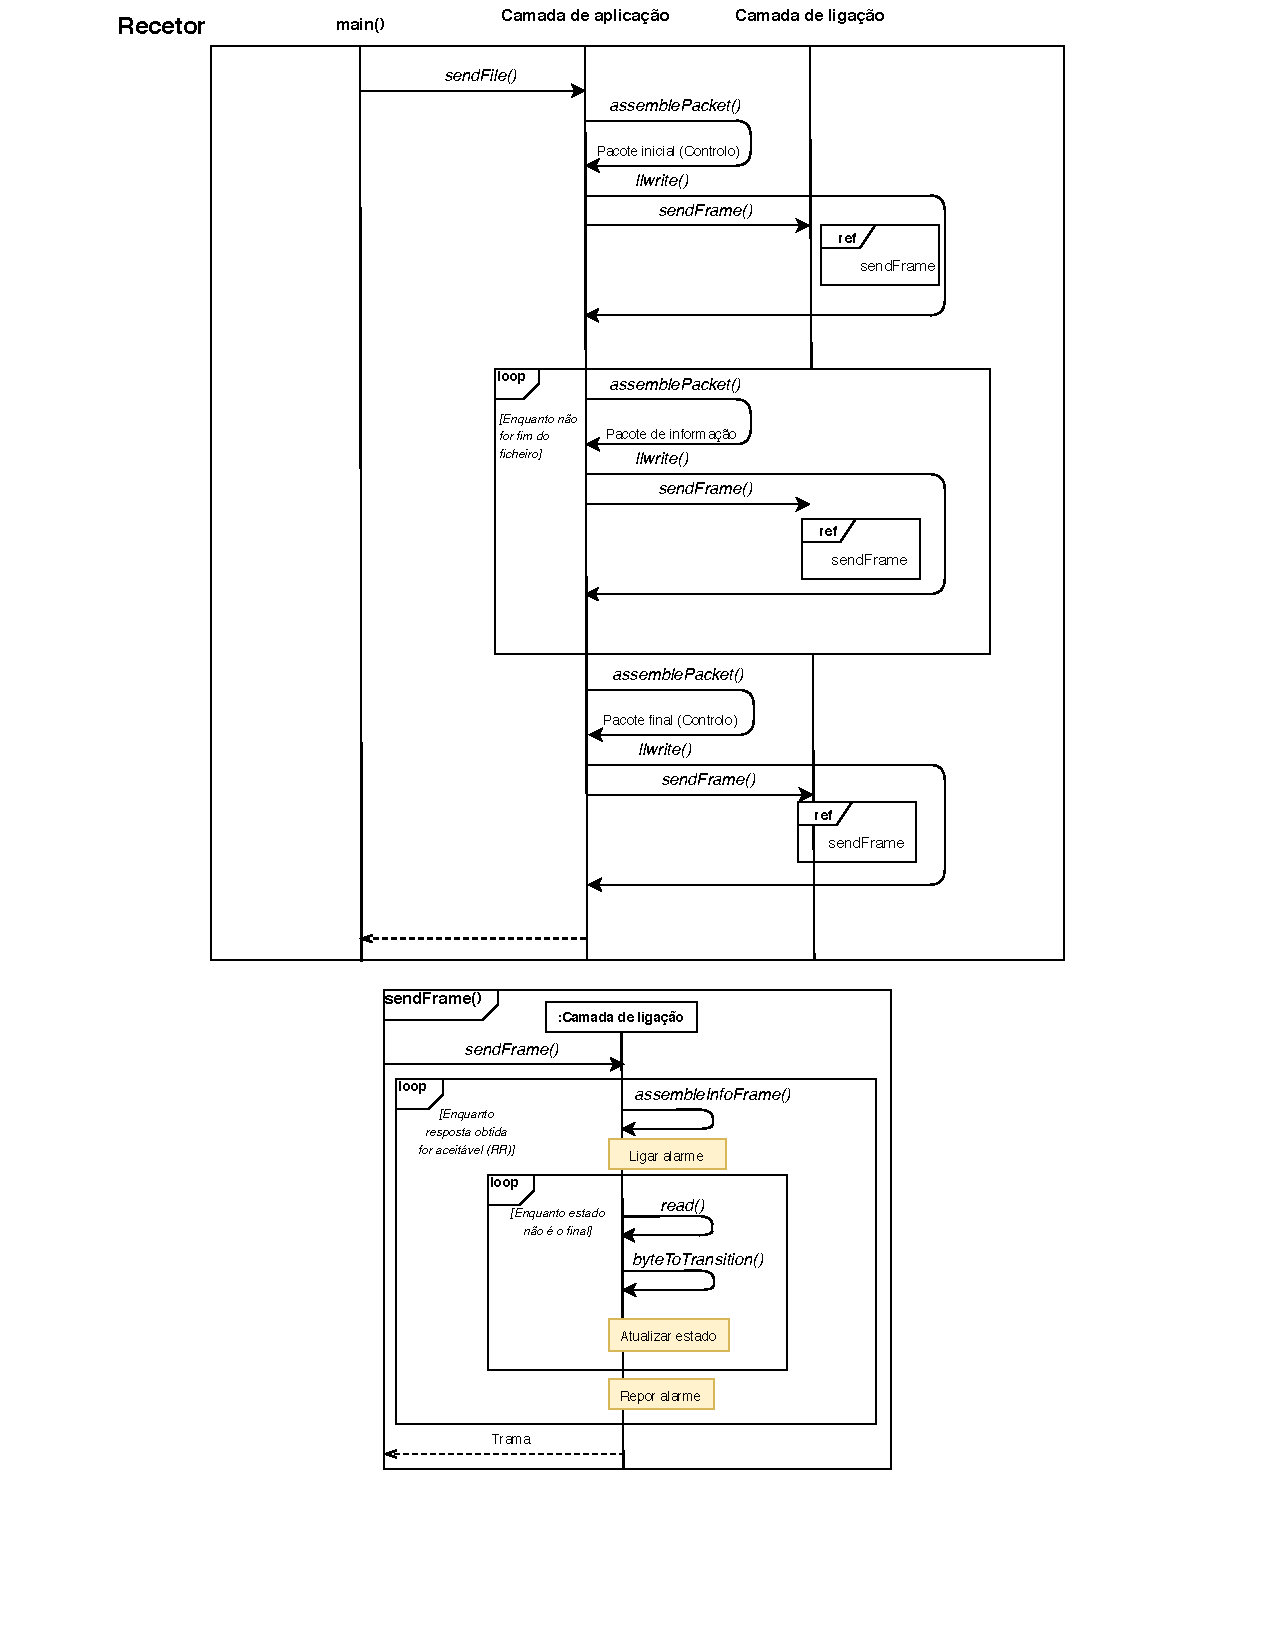
\includegraphics[width=0.9\columnwidth]{images/transmitter.pdf}}
\newpage
\centering{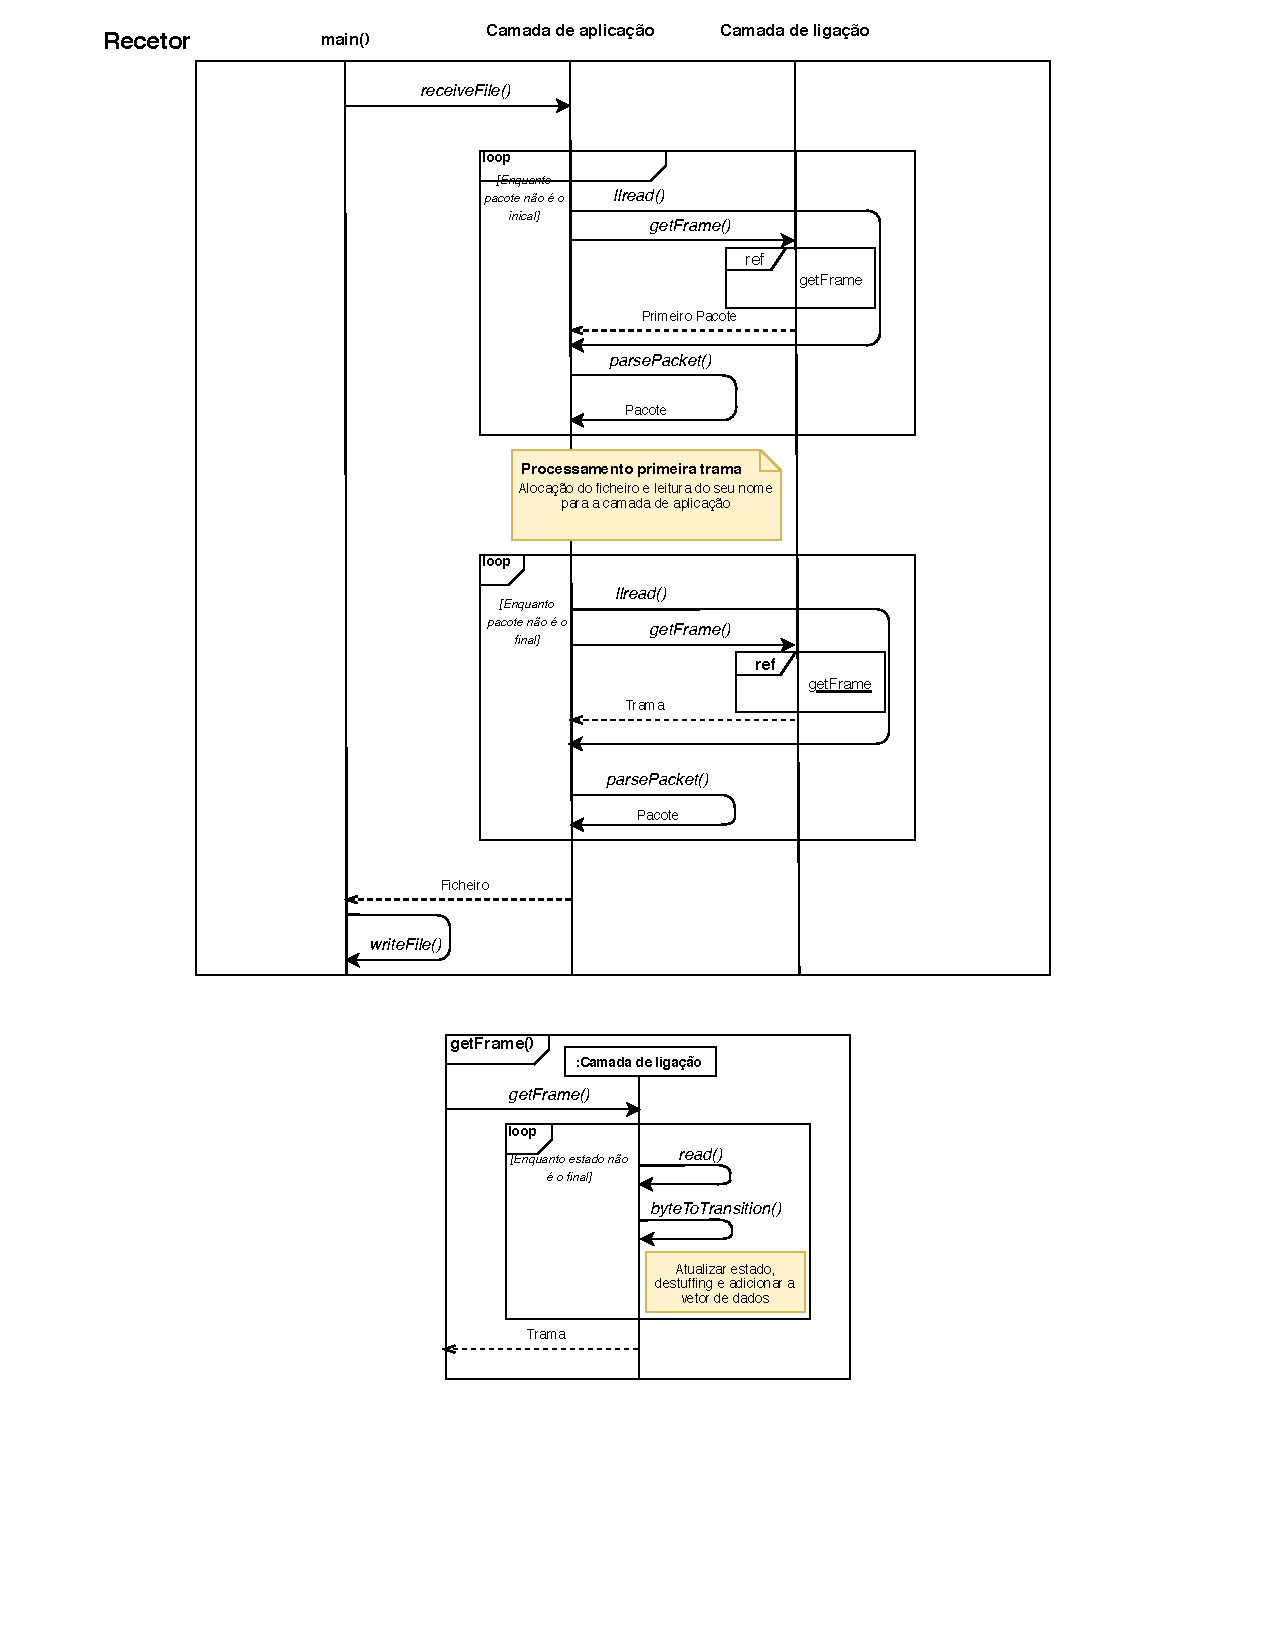
\includegraphics[width=0.9\columnwidth]{images/receiver.pdf}}

\end{document}
